\chapter{Generative Adversarial Networks}

\section{Welcome to GANs}
\href{https://www.youtube.com/watch?v=-h2D0ZWmCM8}{Youtube} \newline

Welcome to this lesson on \textbf{Generative Adversarial Networks} taught by the "Godfather" of GANs, Ian Goodfellow. \newline

By the end of this lesson, you will be able to:

\begin{itemize}
    \item \textbf{Build a generator and a discriminator network}
    \item \textbf{Implement the generator and discriminator loss functions.}
    \item \textbf{Train a GAN on a dataset}
    \item \textbf{Implement some tips and tricks to increase the stability of GAN training}
\end{itemize}
After this lesson, you will have a good understanding of generative adversarial networks and the challenges of successfully training them!

\textbf{Let's get started!}

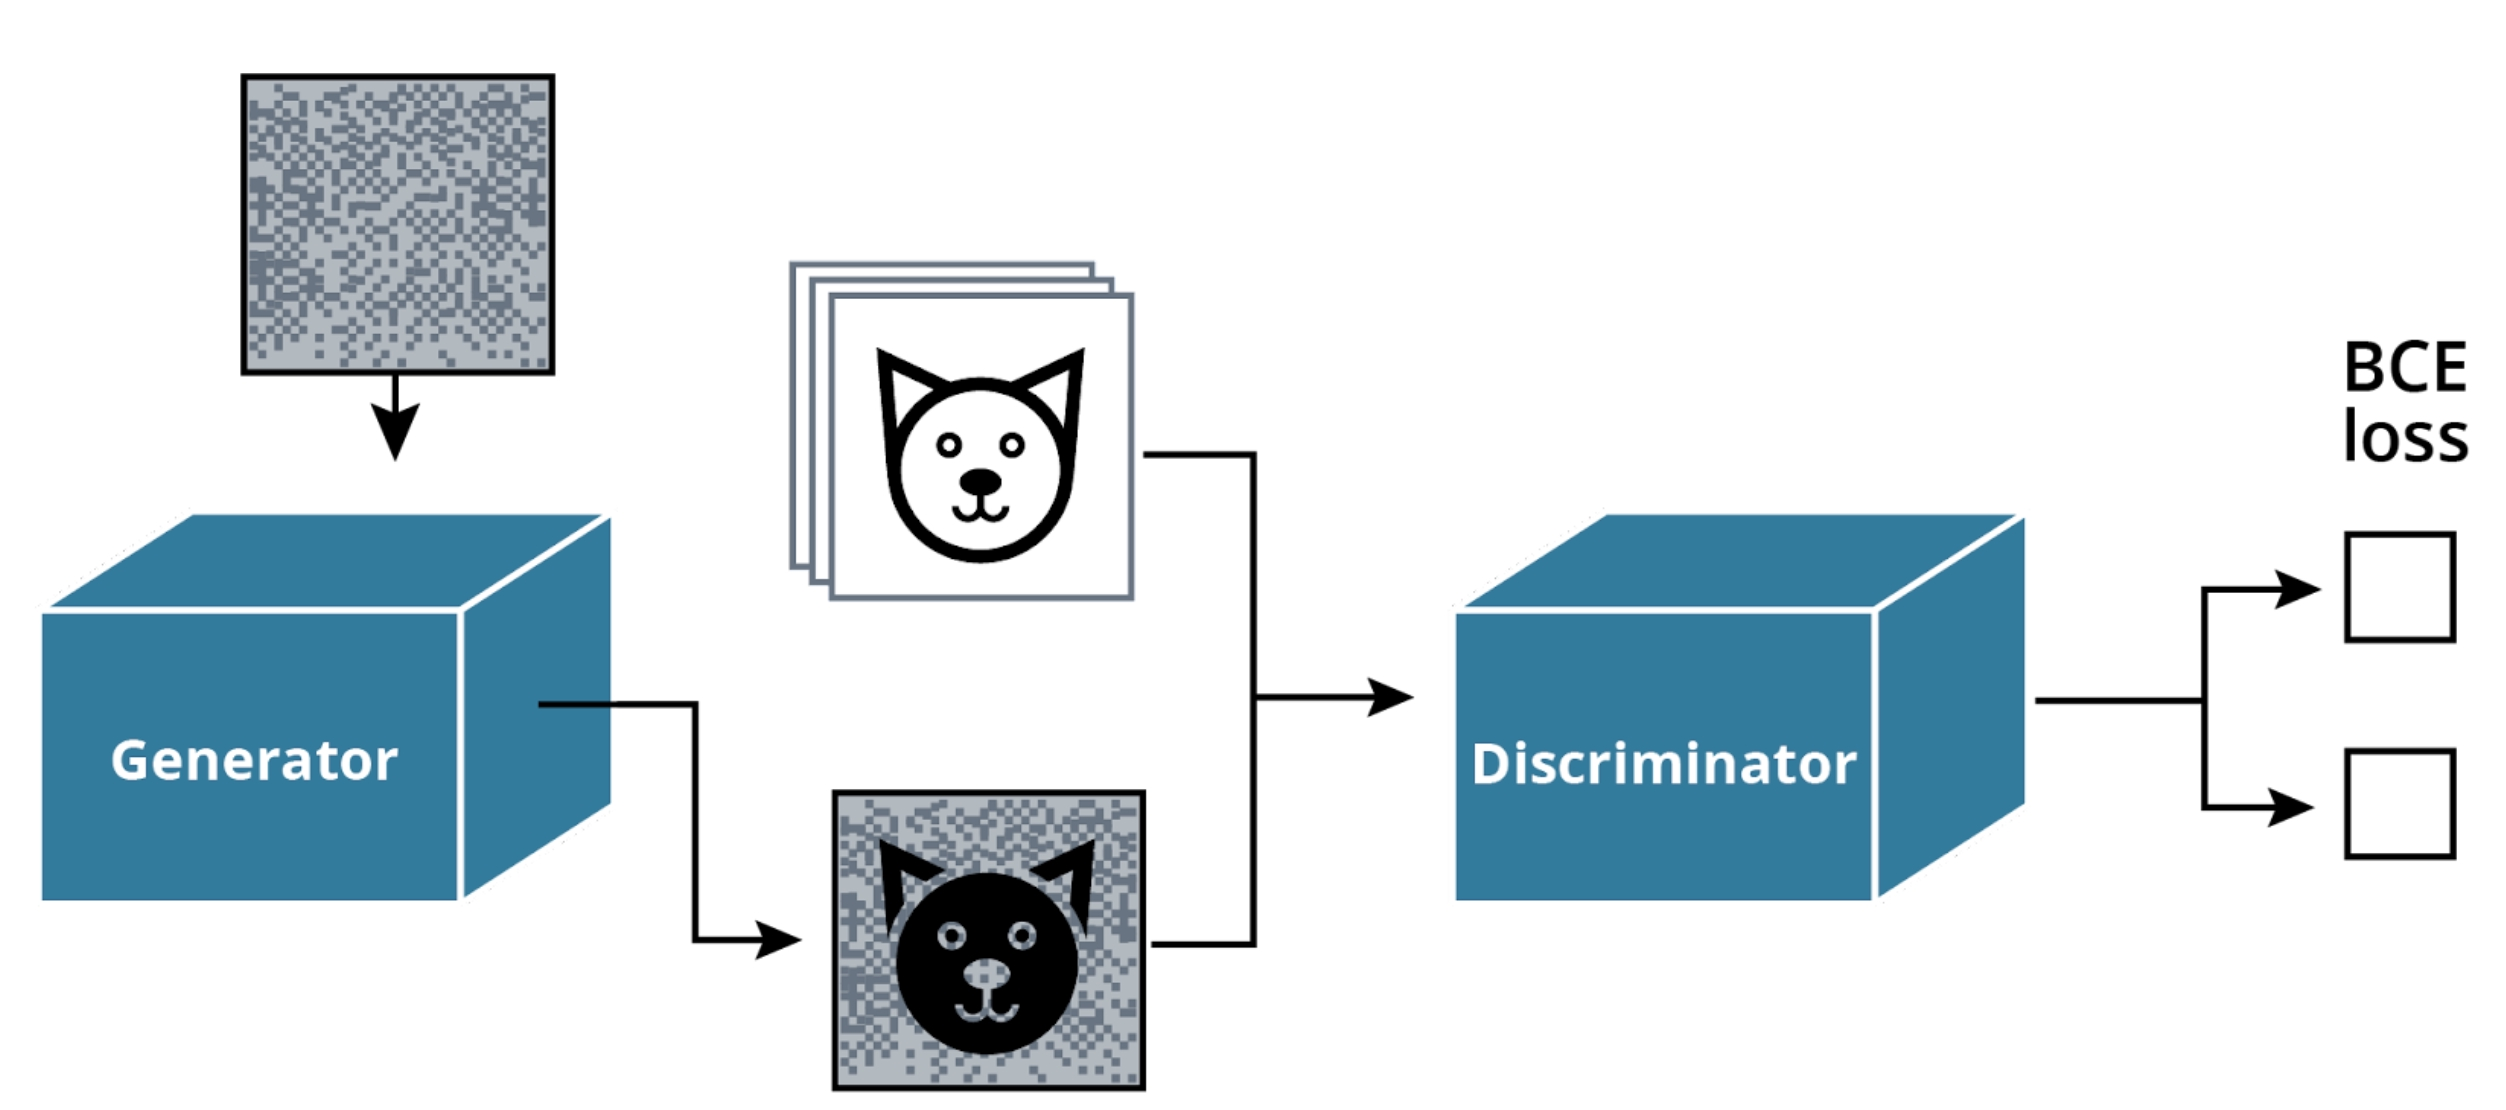
\includegraphics[width=1\linewidth]{img//genAdvNet/screen-shot-2022-05-10-at-9.24.21-am.jpeg}
\captionof{figure}{Schematic representation of GAN architecture}


\section{Lesson Outline}
\href{https://www.youtube.com/watch?v=vu3JV-Va-PM}{Youtube} \newline

In this lesson on \textbf{Generative Adversarial Networks} we will cover the following topics:

\begin{itemize}
    \item Building Generator and Discriminator Networks
    \item Implementing Loss Functions
    \item Training a GAN on a dataset
    \item Implementing techniques to improve GAN training
\end{itemize}

\section{Introducing Ian Goodfellow}
\href{https://www.youtube.com/watch?v=r6tq6-L8Qk0}{Youtube} \newline

Ian Goodfellow is the creator of GANs and has held many roles including:

\begin{itemize}
    \item Senior Research Scientist at Google
    \item Director of Machine Learning at Apple
\end{itemize}
In this lesson, Ian will teach you how to create new \textbf{computer-generated images} that can appear very realistic.

You will find that GANs has real-world application in a number of broad fields including:

\begin{itemize}
    \item \textbf{Computer Vision}
    \item \textbf{The Automotive Industry}
    \item \textbf{Video Gaming}
\end{itemize}
and its implications can be far-reaching.

\section{Applications of GANs}
\href{https://www.youtube.com/watch?v=dW2puRa-yqo}{Youtube} \newline

GANs can be used for a number of broad applications. \newline

\textbf{Visual, Image-Based Applications}

\begin{itemize}
    \item Creating new images
    \item Digital Art
    \item Image to Image Translation
    \item Realistic image training sets
    \item Imitation Learning
\end{itemize}
\textbf{Less Visual Applications}
\begin{itemize}
    \item Predicting the outcome of highly complex physics experiments
    \item Generating adversarial examples
\end{itemize}

\subsubsection{Quiz Question}

What can Generative Adversarial Networks be used for?
\begin{itemize}
    \item \textbf{Generate a new image of a cat}
    \item \textbf{Turn an image of a zebra into a horse}
    \item Image classification
\end{itemize}

\subsection{Additional Resources}

\begin{itemize}
    \item \href{https://arxiv.org/abs/1612.03242}{\textbf{StackGAN: Text to Photo-realistic Image Synthesis with Stacked Generative Adversarial Networks (ArXiv)}}, is an academic paper about using computer vision and pattern recognition to create realistic images.
    \item \href{https://github.com/junyanz/iGAN}{\textbf{iGAN: Interactive Image Generation via Generative Adversarial Networks (GitHub)}}, uses a GANs model to create interactive image generation based on real-time user inputs.
    \item \href{https://video.udacity-data.com/topher/2018/November/5bea23cd_cartoongan/cartoongan.pdf}{\textbf{CartoonGAN: Generative Adversarial Networks for Photo Cartoonization (PDF)}}, is a paper about transforming real-life photos into cartoon-style images.
\end{itemize}

\section{How GANs Work}
\href{https://www.youtube.com/watch?v=--LJlzpsrmA}{Youtube} \newline

\subsection{Image Generation}

\begin{itemize}
    \item \textbf{Fully Visible Belief Networks} – where the model generates an image one pixel at a time. This is also called an \textbf{Autoregressive Model}.
    \item \textbf{Generative Adversarial Networks (GANs)} – where the model generates an entire image in parallel using a differentiable function
\end{itemize}

\subsection{How to Get Realistic Images}
GANs used a combination of neural networks to accomplish the task of image generation:

\begin{itemize}
    \item \textbf{Generator Network –} takes random input through a differentiable function to transform and reshape it to have a recognizable structure. The output is a realistic image.
\end{itemize}

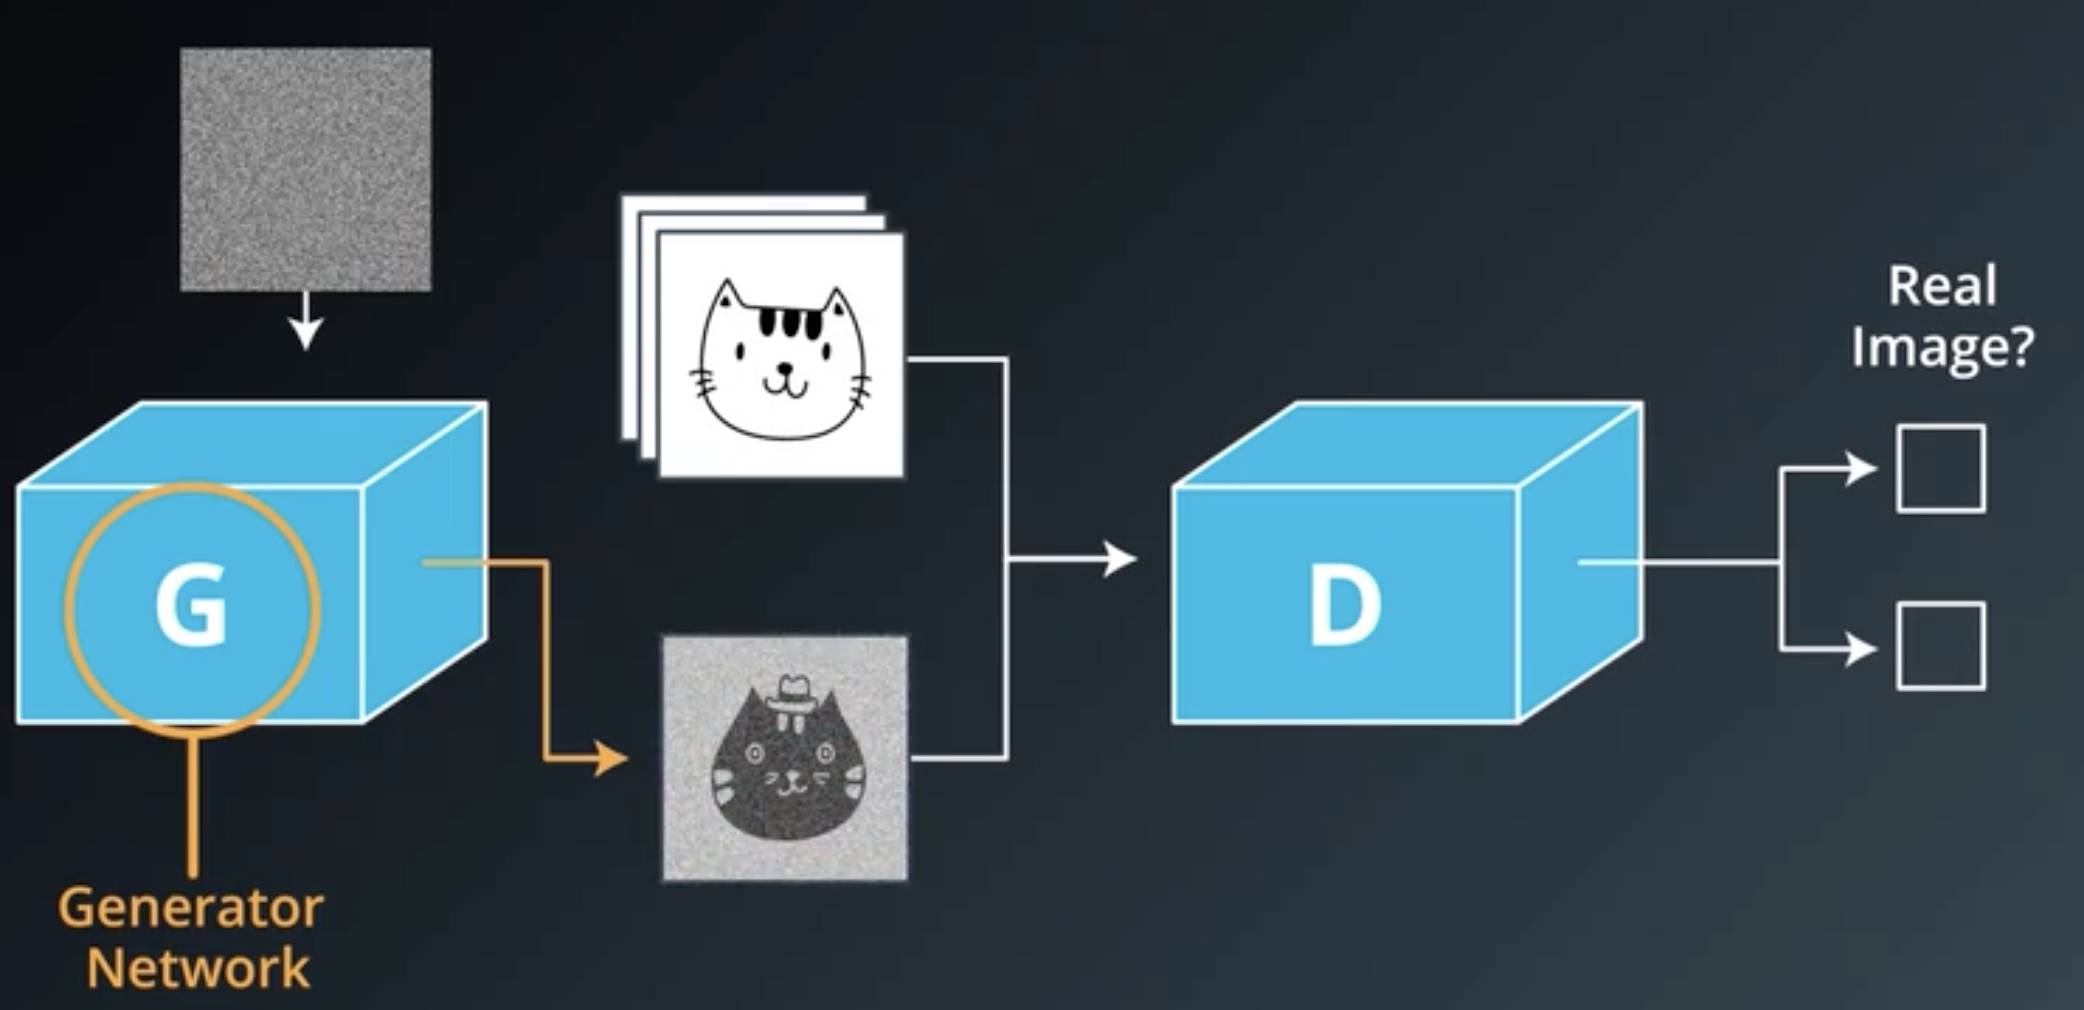
\includegraphics[width=0.5\linewidth]{img//genAdvNet/screen-shot-2022-06-30-at-7.04.47-pm.jpeg}
\captionof{figure}{Generators create new images based on a dataset}

Unlike training a supervised learning model, when training a generator model, there is no classification/label to associate with each image. It creates additional images based on a probability distribution.

\begin{itemize}
    \item \textbf{Discriminator Network –} is a regular neural net classifier that learns to guide the generator network by outputting the probability that the input is real. Fake images are 0 and real images are 1.
\end{itemize}

The generator network is forced to produce more realistic images to "fool" the discriminator network.

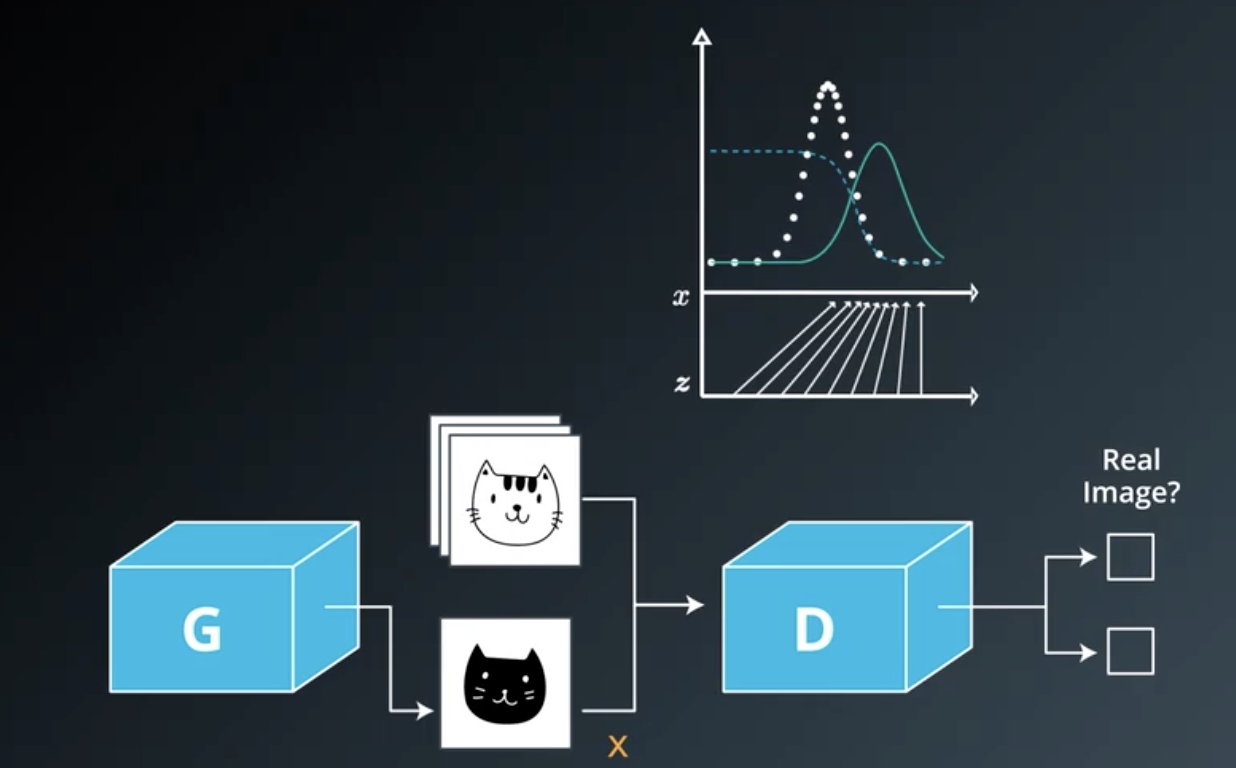
\includegraphics[width=0.5\linewidth]{img//genAdvNet/screen-shot-2022-06-30-at-7.07.48-pm.jpeg}
\captionof{figure}{Discriminators determine the probability of an image being "real" or "fake"}

\subsubsection{Additional Resources}
Here's the same sentence with a descriptive link text for the hyperlink: \newline

Check out Ian's original paper on \href{https://arxiv.org/pdf/1406.2661.pdf}{\textbf{Generative Adversarial Nets (ArXiv PDF)}}[1].

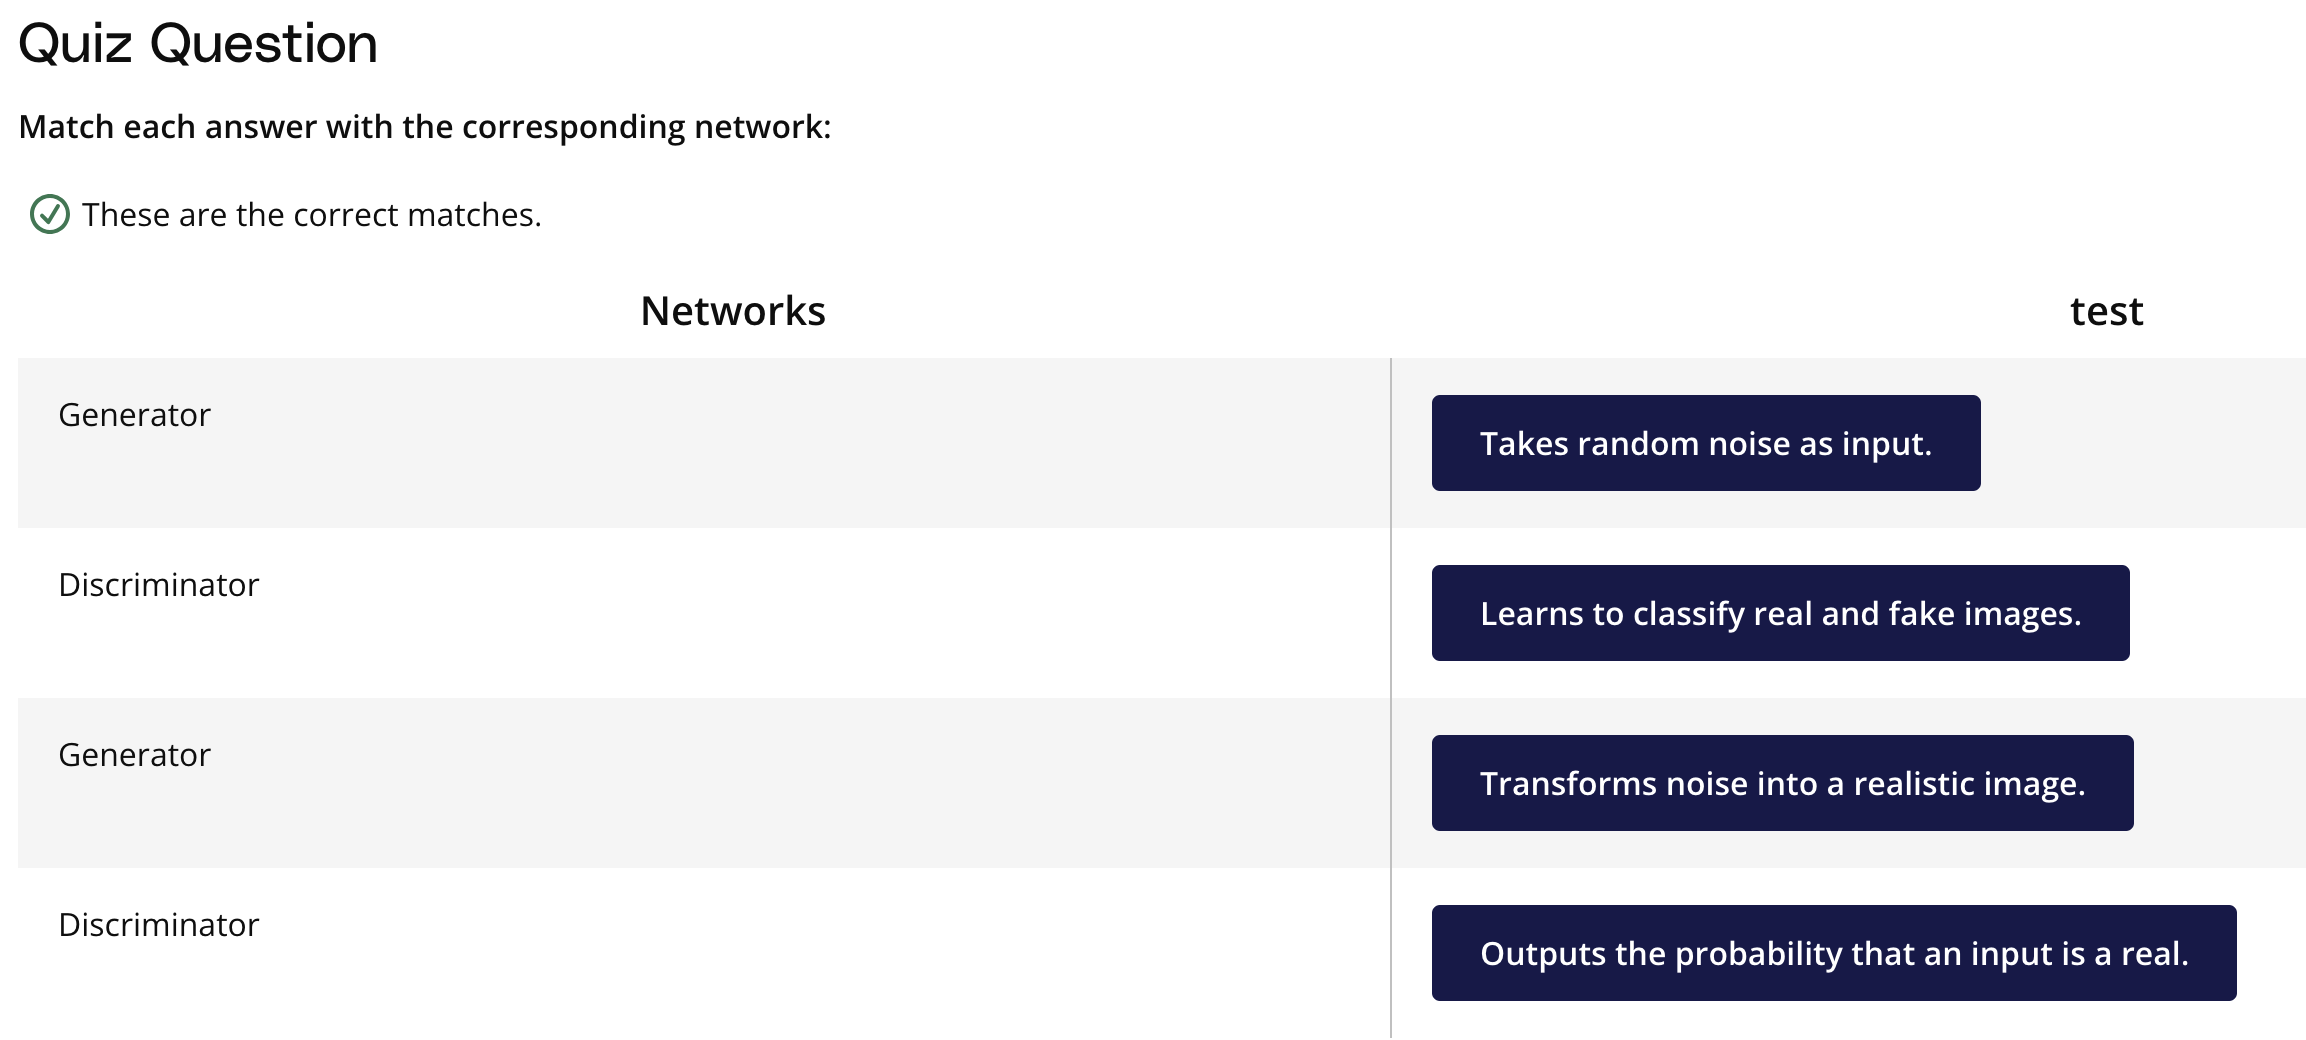
\includegraphics[width=1\linewidth]{img//genAdvNet//gan/image.png}

Good job! Training a GAN is like watching a competition between two networks, the discriminator and the generator. The generator tries to fool the discriminator by creating realistic images and the discriminator tries to identify which money is fake and which one is real.

\subsection{Citations}
Following is the full citation for the paper referenced on this page:

\begin{itemize}
    \item \textbf{[1]} I. Goodfellow, J. Pouget-Abadie, M. Mirza, et al, "\textit{Generative Adversarial Nets}", Departement d’informatique et de recherche operationnelle Universite de Montreal [Online], Available: \href{https://arxiv.org/pdf/1406.2661.pdf}{\textbf{https://arxiv.org/pdf/1406.2661.pdf}}. [Accessed June 28, 2022].
\end{itemize}

\section{Discriminator and Generator
implementation}\label{discriminator-and-generator-implementation}

In this notebook, you will implement the generator and discriminator
models. These models will be use in the last exercise of this lesson to
train your first GAN network!

\subsection{Discriminator}\label{discriminator}

The discriminator network is going to be a pretty typical linear
classifier. To make this network a universal function approximator,
we'll need at least one hidden layer, and these hidden layers should
have one key attribute: \textgreater{} All hidden layers will have a
\href{https://pytorch.org/docs/stable/nn.html\#torch.nn.LeakyReLU}{Leaky ReLu} activation function applied to their outputs.

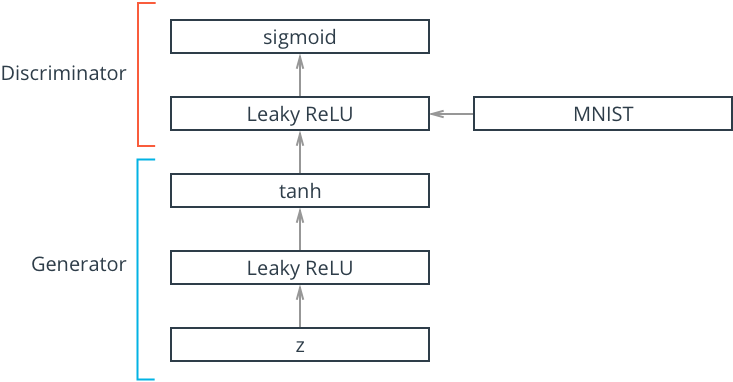
\includegraphics[width=0.5\linewidth]{img//genAdvNet//gan/gan_network.png}

\paragraph{Leaky ReLu}\label{leaky-relu}

We should use a leaky ReLU to allow gradients to flow backwards through
the layer unimpeded. A leaky ReLU is like a normal ReLU, except that
there is a small non-zero output for negative input values.

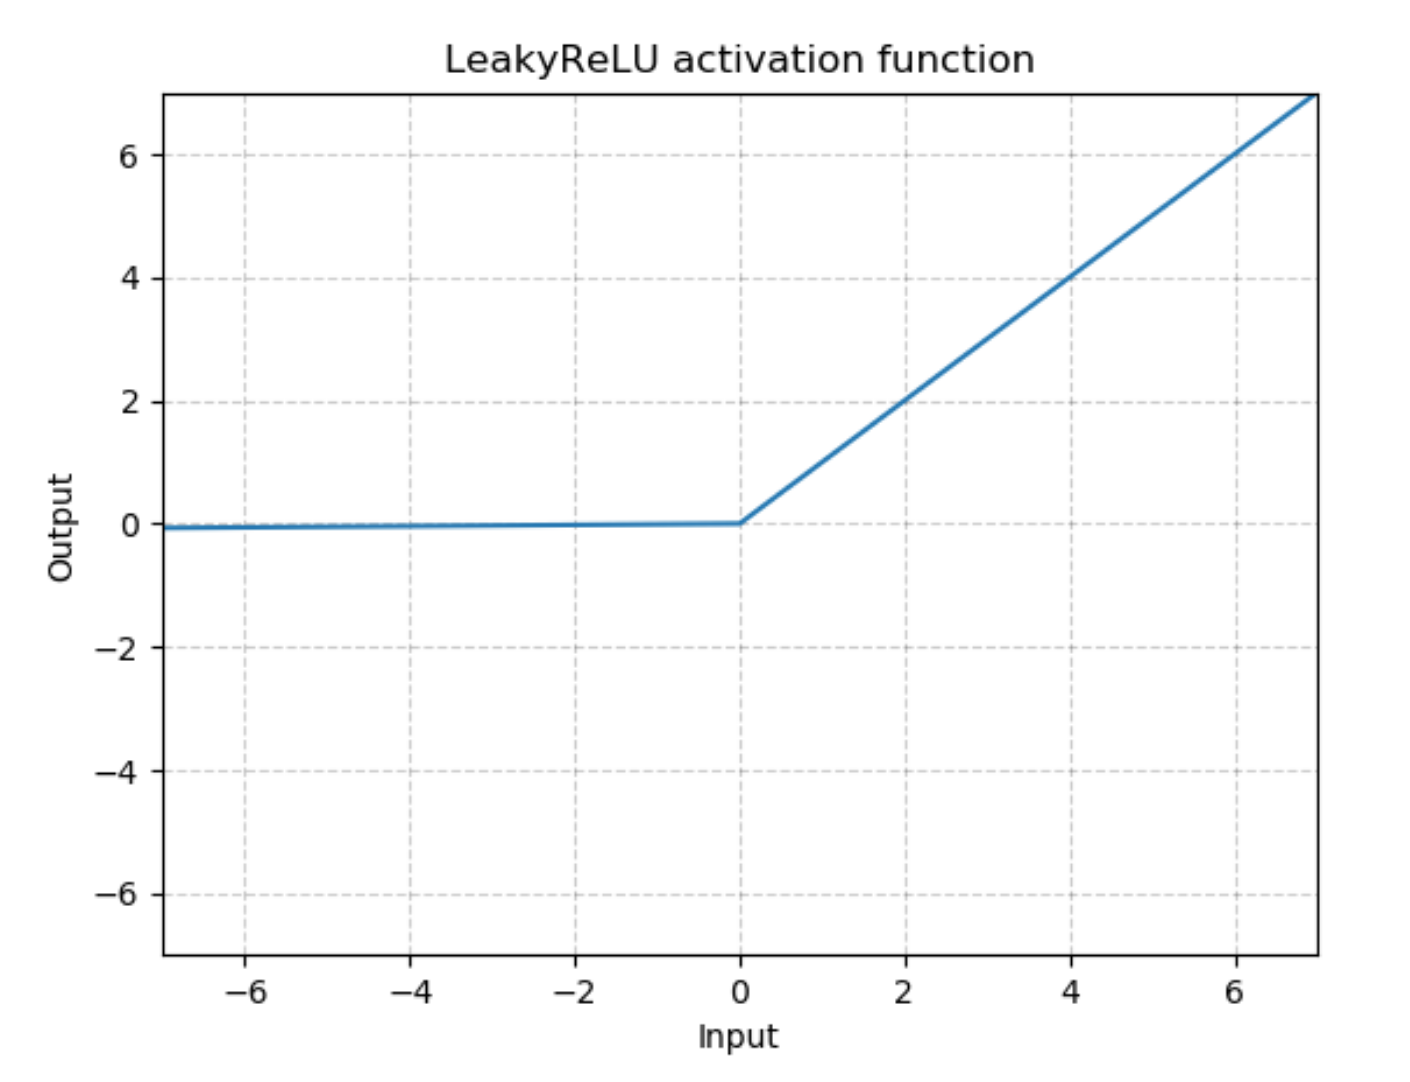
\includegraphics[width=0.5\linewidth]{img//genAdvNet//gan/leaky_relu.png}

\paragraph{Output}\label{output}

We'll also take the approach of using a more numerically stable loss
function on the outputs. Recall that we want the discriminator to output
a value 0-1 indicating whether an image is \emph{real or fake}.
\textgreater{} We will ultimately use
\href{https://pytorch.org/docs/stable/nn.html\#bcewithlogitsloss}{BCEWithLogitsLoss},
which combines a \lstinline{sigmoid} activation function
\textbf{and} binary cross entropy loss in one function.

So, our final output layer should not have any activation function
applied to it.

\paragraph{Structure}\label{structure}

The discriminator takes a high dimensional input (for example, an image)
and outputs a single score value. Linear layers in the discriminator
should have a number of neurons such that the dimensions of their output
is smaller than the dimension of their input.

\subsubsection{First exercise}\label{first-exercise}

Implement a discriminator network. Your network should: 
\begin{itemize}
    \item use fully connected layer and leaky relu
    \item output a single logit
    \item take a image asinput
\end{itemize}
\begin{lstlisting}[language=Python]
import torch
import torch.nn as nn

import tests
\end{lstlisting}

\begin{lstlisting}[language=Python]
class Discriminator(nn.Module):
    """
    Discriminator model:
    args: 
    - input_dim: dimension of the input data. For example, for a 28 by 28 grayscale image, the input size is 784
    - hidden_dim: a parameter that controls the dimensions of the hidden layers. 
    """
    def __init__(self, input_dim: int, hidden_dim: int):
        super(Discriminator, self).__init__()
        self.model = nn.Sequential(
            # Flatten image
            nn.Flatten(),
            # Hidden layers, activations & dropout
            nn.Linear(input_dim, hidden_dim),
            nn.LeakyReLU(0.1),
            nn.Dropout(0.2),
            nn.Linear(hidden_dim, hidden_dim // 2),
            nn.LeakyReLU(0.1),
            nn.Dropout(0.2),
            nn.Linear(hidden_dim // 2, hidden_dim // 4),
            nn.LeakyReLU(0.1),
            nn.Dropout(0.2),
            nn.Linear(hidden_dim // 4, 1)
        )
        #### 
        # IMPLEMENT HERE
        ####
        
    def forward(self, x: torch.Tensor) -> torch.Tensor:
        #### 
        # IMPLEMENT HERE
        ####
        return self.model(x)
\end{lstlisting}

\begin{lstlisting}[language=Python]
# for a 28x28 grayscale image flattened, the input dim is 784
input_dim = 784
hidden_dim = 256

discriminator = Discriminator(input_dim, hidden_dim)
tests.check_discriminator(discriminator, input_dim)
\end{lstlisting}

\begin{lstlisting}
Congrats, you successfully implemented your discriminator
\end{lstlisting}

\subsection{Generator}\label{generator}

The generator network will be almost exactly the same as the
discriminator network, except that we're applying a
\href{https://pytorch.org/docs/stable/nn.html\#tanh}{tanh activation
function} to our output layer.

\paragraph{tanh Output}\label{tanh-output}

The generator has been found to perform the best with \(tanh\) for the
generator output, which scales the output to be between -1 and 1,
instead of 0 and 1.

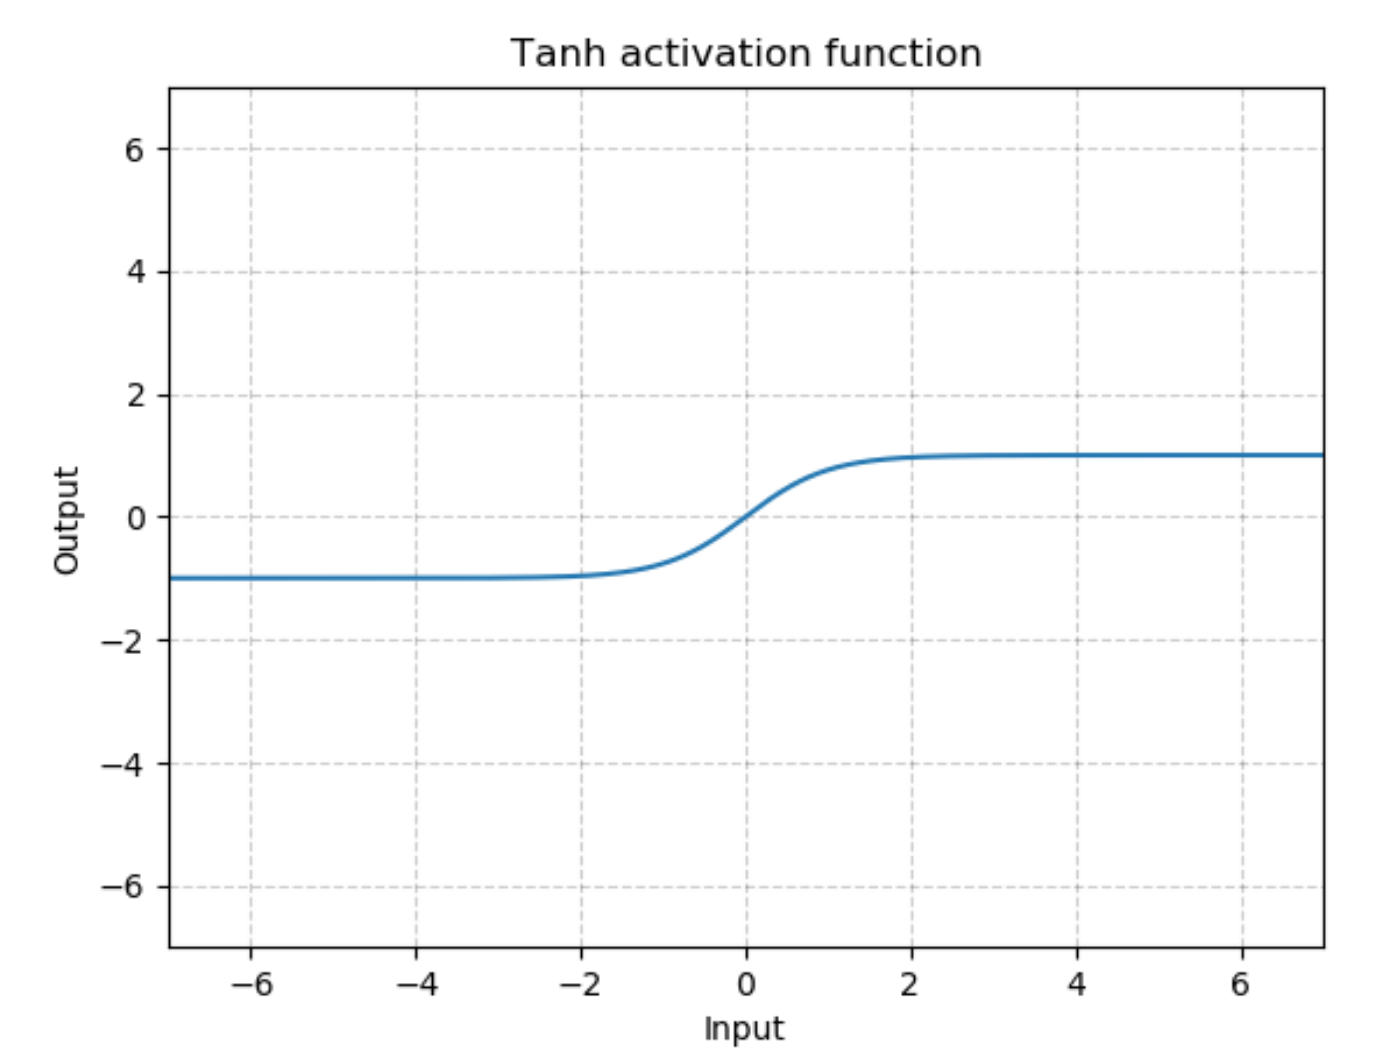
\includegraphics[width=0.5\linewidth]{img//genAdvNet//gan/tanh_fn.png}

Recall that we also want these outputs to be comparable to the
\emph{real} input pixel values, which are read in as normalized values
between 0 and 1. \textgreater{} So, we'll also have to \textbf{scale our
real input images to have pixel values between -1 and 1} when we train
the discriminator.

\subsection{Second Exercise}\label{second-exercise}

Implement a generator network. Your network should: * use fully
connected, leaky relu and tanh layers * take a latent as input * output
a vector (we will later reshape it as an image)

\begin{lstlisting}[language=Python]
class Generator(nn.Module):
    def __init__(self, latent_dim: int, hidden_dim: int, output_size: int):
        super(Generator, self).__init__()
        self.model = nn.Sequential(
            # Hidden layers, activations & dropout
            nn.Linear(latent_dim, hidden_dim),
            nn.LeakyReLU(0.1),
            nn.Dropout(0.2),
            nn.Linear(hidden_dim, hidden_dim * 2),
            nn.LeakyReLU(0.1),
            nn.Dropout(0.2),
            nn.Linear(hidden_dim * 2, hidden_dim * 4),
            nn.LeakyReLU(0.1),
            nn.Dropout(0.2),
            # Final layer
            nn.Linear(hidden_dim * 4, output_size),
            # Final tanh function to output layer
            nn.Tanh()
        )
        #### 
        # IMPLEMENT HERE
        ####

    def forward(self, x: torch.Tensor) -> torch.Tensor:
        #### 
        # IMPLEMENT HERE
        ####
        return self.model(x)
\end{lstlisting}

\begin{lstlisting}[language=Python]
latent_dim = 128
hidden_dim = 256
output_dim = 784

generator = Generator(latent_dim, hidden_dim, output_dim)
tests.check_generator(generator, latent_dim, output_dim)
\end{lstlisting}

\begin{lstlisting}
Congrats, you successfully implemented your generator
\end{lstlisting}

\section{Exercise Part 1: Solution}
\href{https://www.youtube.com/watch?v=Wat3QCqs6Is}{Youtube}

\section{Games and Equilibria}
\href{https://www.youtube.com/watch?v=Vpzm8r8C2CY}{Youtube}

\subsection{Adversarial}

In GANs, \textbf{adversarial} means that two networks, the generator and the discriminator, compete with each other for improved image generation. \newline

This "competition" between the networks is based on \textbf{Game Theory}. \newline

\textbf{Game Theory –} a form of applied mathematics used to model cooperation and conflict between rational agents in any situation \newline

\href{https://www.youtube.com/watch?v=O0J6kzhjf4M}{Youtube}
\subsection{Equilibria and GANs}

Most ML models are based on optimization and follow the general pattern of

\begin{enumerate}
    \item Determine model parameters
    \item Have a cost function of these parameters
    \item Minimize the cost
\end{enumerate}
GANs are different because there are two players, the generator and the discriminator, and each player has its own cost. The "game" is therefore defined by a value function.

\begin{itemize}
    \item The \textbf{generator wants to minimize} the value function.
    \item The \textbf{discriminator wants to maximize} the value function.
    \item The \textbf{saddle point} is when equilibrium is reached, a point in the parameters of both players that is simultaneously a local minimum for each player's costs with respect to that player's parameters.
\end{itemize}
A key learning problem for GANs is finding the equilibrium of a game involving cost functions that are:

\begin{itemize}
    \item High dimensional
    \item Continuous
    \item Non-convex
\end{itemize}

\subsubsection{Quiz Question}
Which of the following statements are true?
\begin{itemize}
    \item \textbf{Training a GAN is equivalent to playing a game where both networks are competing with each other.}
    \item When training a GAN, after some time, the equilibrium is always reached.
    \item Game Theory is a subfield of deep learning invented to describe GANs training.
    \item The GAN equilibrium is reached when the discriminator loss reaches 0
\end{itemize}


\subsection{Additional Reading}

A very famous example of Game Theory is the Prisoner Dilemma. This \href{https://www.youtube.com/watch?v=t9Lo2fgxWHw}{\textbf{explanatory video on the Prisoner's Dilemma}} explains this game very well. A few others concepts are keys to understand game theory:

\begin{itemize}
    \item \href{https://en.wikipedia.org/wiki/Nash_equilibrium}{\textbf{Nash equilibrium}}: an equilibrium reached when neither player gain anything by changing their strategies. In the Prisoner Dilemma's game, the Nash Equilibrium is attained when both players decide to betray each other
    \item \href{https://en.wikipedia.org/wiki/Pareto_efficiency}{\textbf{Pareto optimality}}: a strategy is Pareto optimal when neither player can be better off without another player being negatively affected. In the Prisoner Dilemma's game, both players deciding to not betray each other is Pareto optimal.
\end{itemize}

\section{Tips for Training GANs}
\href{https://www.youtube.com/watch?v=JXfgLuCLFM8}{Youtube}

\subsection{Good Architecture}

\textbf{Fully Connected Architecture} can be used for simple tasks that meet the following criteria:

\begin{enumerate}
    \item No convolution
    \item No recurrence
    \item The generator and discriminator have a least one hidden layer
\end{enumerate}
\textbf{Leaky ReLU} helps to make sure that the gradient can flow through the entire architecture and is a popular choice for hidden layer activation functions. \newline

The \textbf{Hyperbolic Tangent} activation function is a popular output choice for the generator and means data should be scaled to the interval from -1 to +1. \newline

A \textbf{Sigmoid Unit} is used to enforce the constraint that the output of the discriminator is a probability.

\subsection{Design Choice}

One of the design choices from the DCGAN architecture is \textbf{Adam}, an optimization algorithm. \newline

A common error is that people forget to use a numerically stable version of \textbf{cross-entropy}, where the loss is computed using the \textbf{logits}. \newline

\textbf{Logits} – the values produced by the discriminator right before the \textbf{sigmoid}.

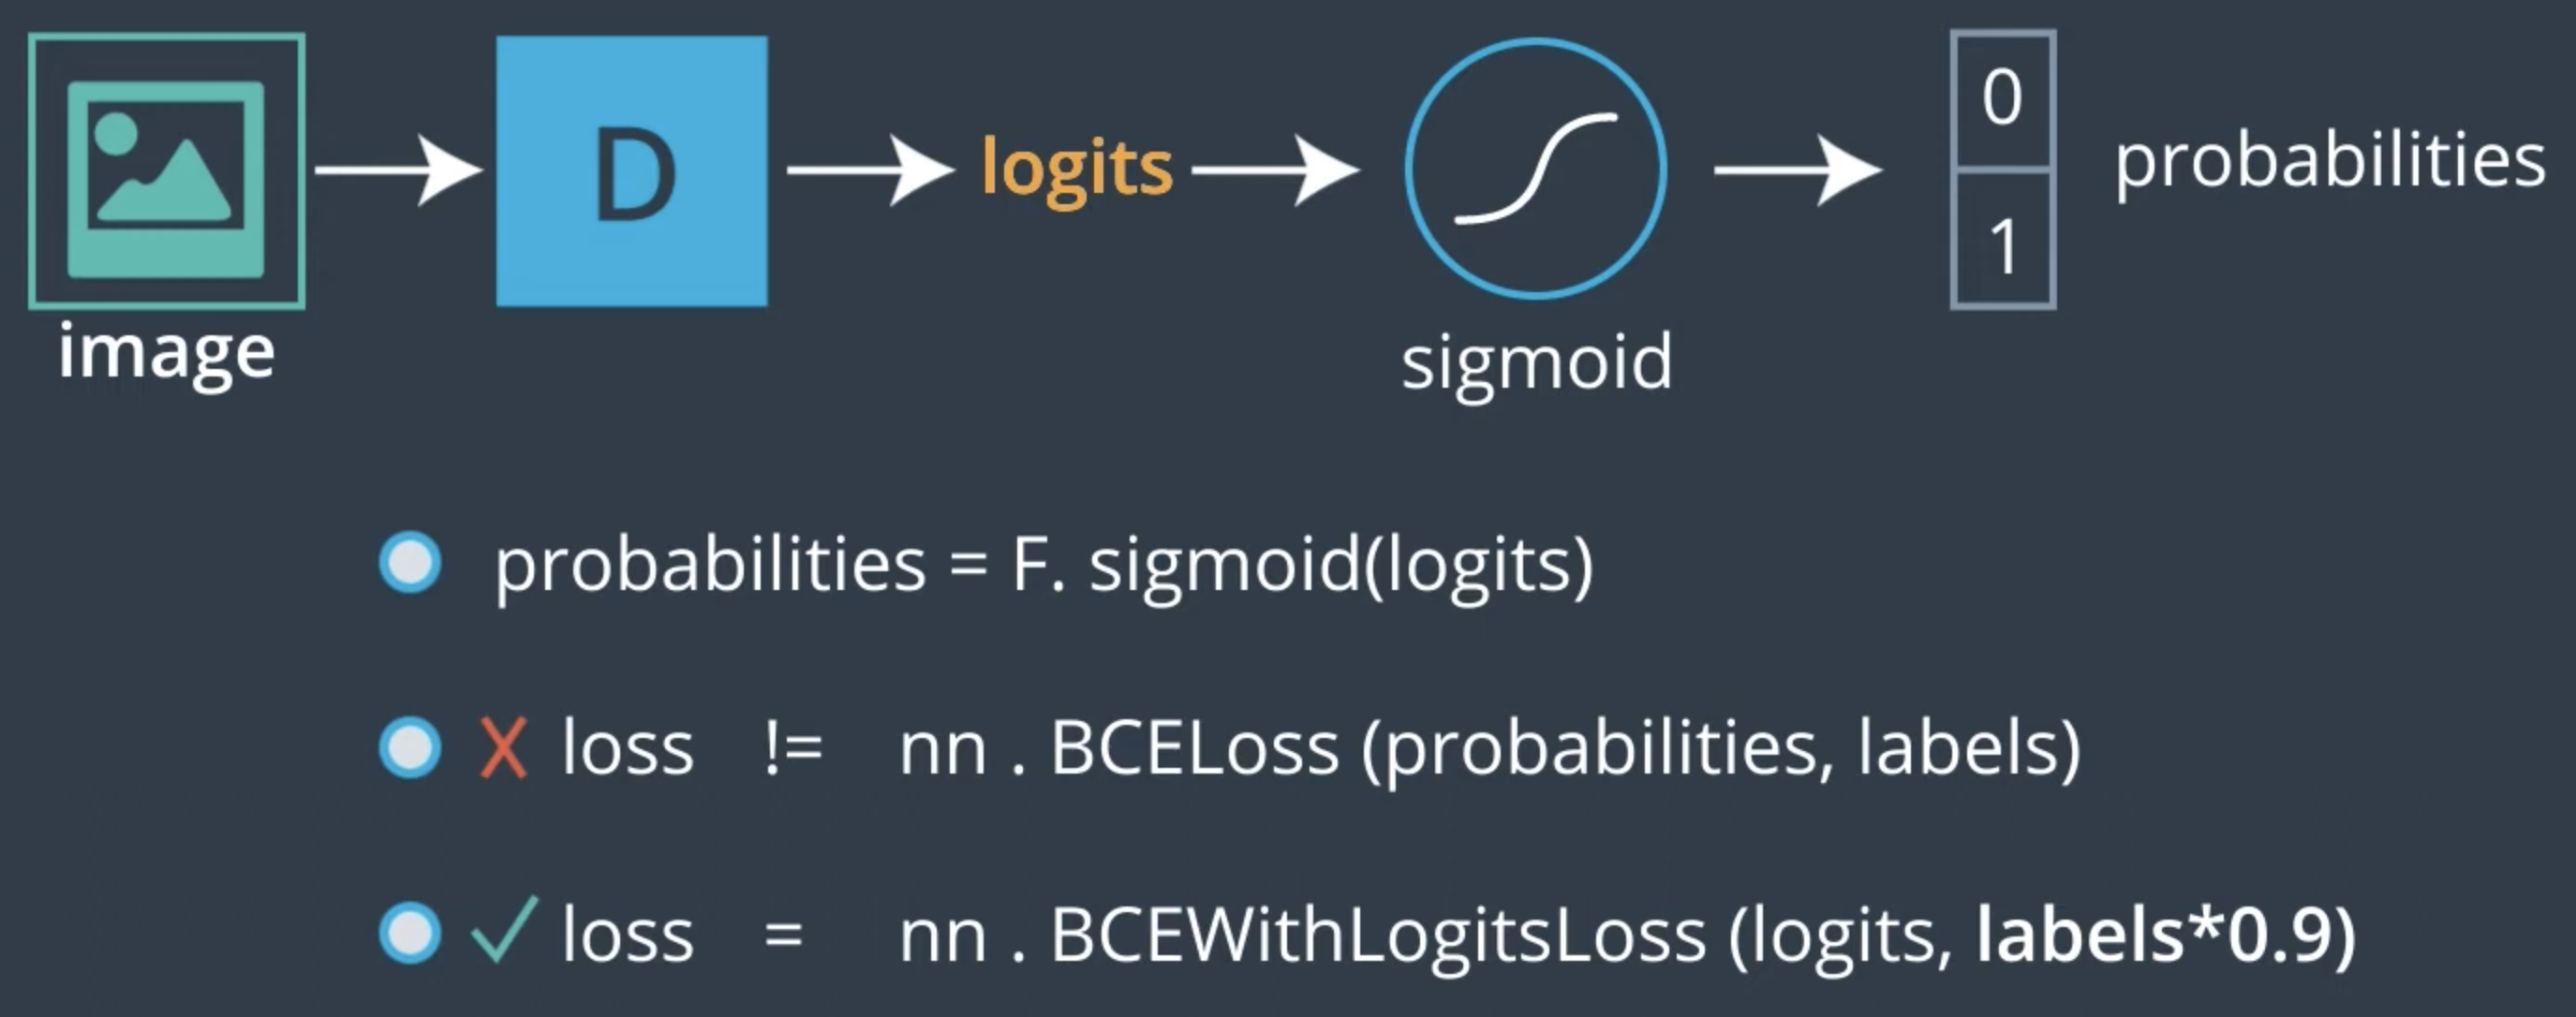
\includegraphics[width=1\linewidth]{img//genAdvNet//gan/numericallyStableCrossEntropy.png}
\captionof{figure}{Numerically Stable Cross-Entropy}
\label{fig:numericallyStableCE}

\subsection{Tips for Training}

\begin{enumerate}
    \item A simple trick is to multiply the 0 or 1 labels by a number a bit less than 1. This is a GANs-specific label smoothing strategy similar to that used to regularize normal classifiers (see \autoref{fig:numericallyStableCE}).
    \item For the generator loss, minimize cross-entropy with the labels flipped.
\end{enumerate}

\href{https://www.youtube.com/watch?v=iMvn7l6HztI&t=1s}{Youtube}
\subsection{Scaling GANs}

\textbf{Convolutional Neural Networks (CNN)} are needed to scale GANs to work on larger images. Scaling GANs relies on an understanding of:

\begin{itemize}
    \item \textbf{Classifier Convolutional Net –} starting with a tall and wide feature map and moving to very short and narrow feature maps
    \item \textbf{Generator Net} – starting with short and narrow feature maps and moving to a wide and tall image
    \item \textbf{Batch Normalization} – on potentially every layer except the output layer of the generator and the input layer of the discriminator
\end{itemize}

\subsection{Improved Training Techniques for GANs}

The paper, \href{https://video.udacity-data.com/topher/2018/November/5bea0c6a_improved-training-techniques/improved-training-techniques.pdf}{\textbf{Improved Techniques for Training GANs (PDF)}}, describes improved training techniques for GANs!

\subsection{Quiz}

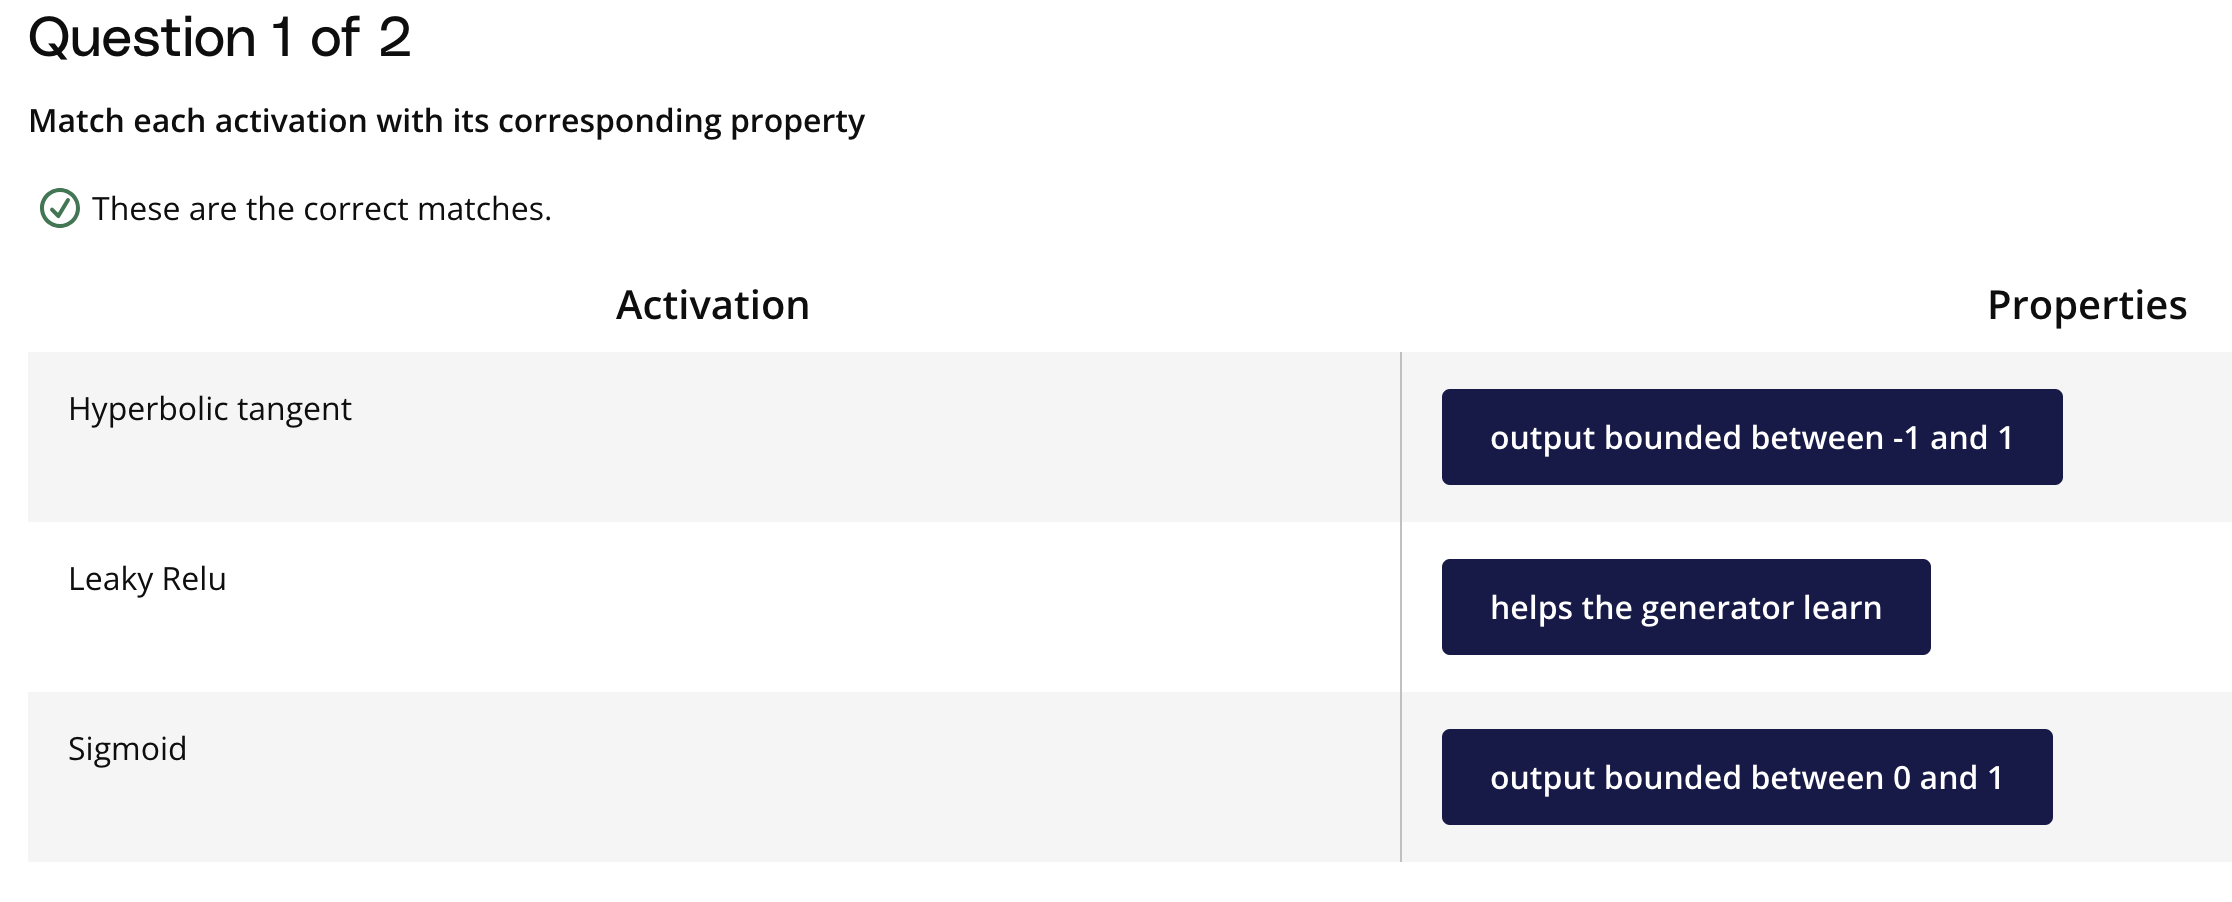
\includegraphics[width=1\linewidth]{img//genAdvNet//gan/quiz2.png}

Which of the following statements are true? (There are multiple correct choices - check all that apply)
\begin{itemize}
    \item \textbf{The binary cross entropy (BCE) loss can be used to train both the generator and the discriminator.}
    \item \textbf{Label smoothing consists in multiplying the labels by a float smaller than 1.}
    \item \textbf{When training the generator, the BCE loss is used with flipped labels (fake = 1, real = 0)}
    \item \textbf{The BCE loss is only one of the possible loss functions to train a GAN. Many other options exist.}
\end{itemize}

\begin{center}\rule{0.5\linewidth}{0.5pt}\end{center}

\subsection{Discriminator and Generator
Losses}\label{discriminator-and-generator-losses}

Now we need to calculate the losses.

\subsubsection{Discriminator Losses}\label{discriminator-losses}

\begin{quote}
\begin{itemize}
\item For the discriminator, the total loss is the sum of the losses for
  real and fake images,
  \lstinline{d_loss = d_real_loss + d_fake_loss}.
\item  Remember that we want the discriminator to output 1 for real images
  and 0 for fake images, so we need to set up the losses to reflect
  that.
\end{itemize}
\end{quote}

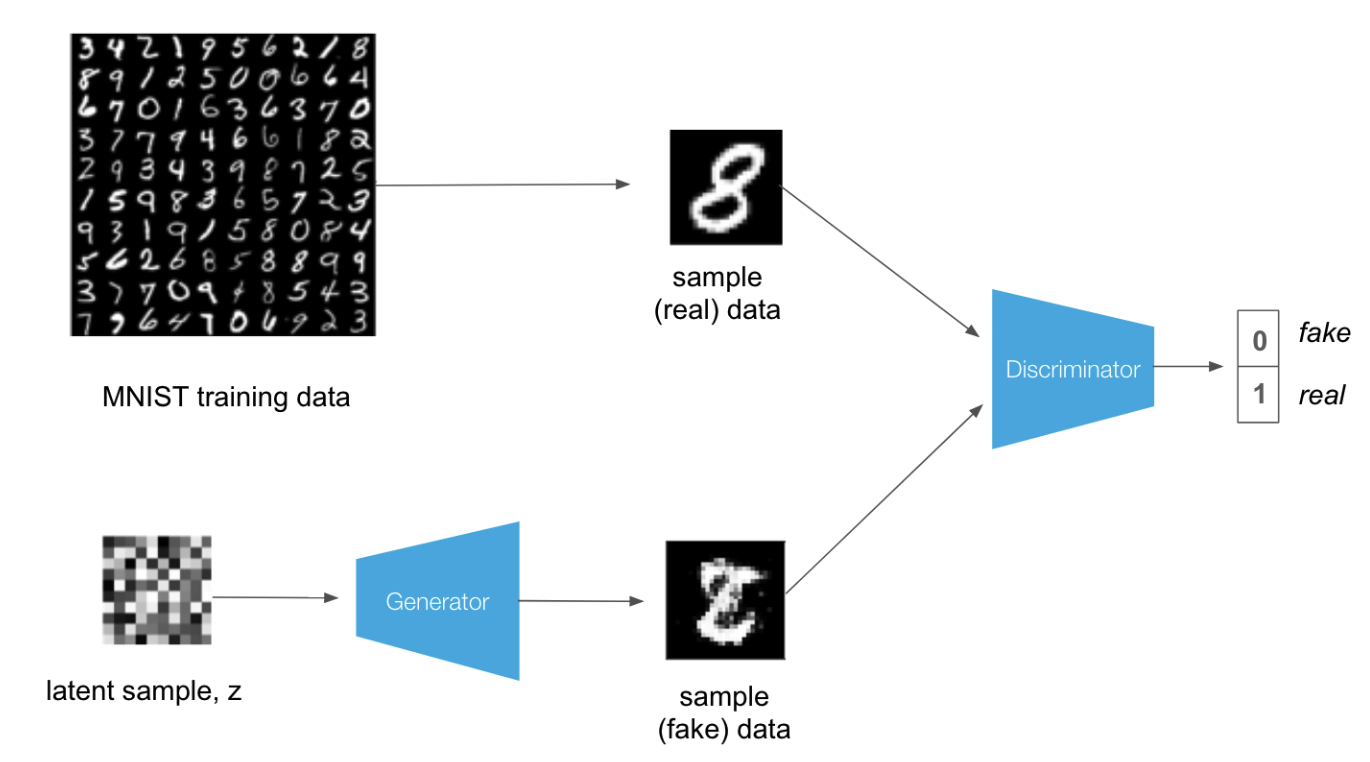
\includegraphics[width=1\linewidth]{img//genAdvNet//gan/part2_screengrab.png}

The losses will by binary cross entropy loss with logits, which we can
get with
\href{https://pytorch.org/docs/stable/nn.html\#bcewithlogitsloss}{BCEWithLogitsLoss}.
This combines a \lstinline{sigmoid} activation function
\textbf{and} and binary cross entropy loss in one function.\newline

For the real images, we want
\lstinline{D(real_images) = 1}. That is, we want the
discriminator to classify the the real images with a label = 1,
indicating that these are real. To help the discriminator generalize
better, the labels are \textbf{reduced a bit from 1.0 to 0.9}. For this,
we'll use the parameter \lstinline{smooth}; if True, then
we should smooth our labels by a factor of 0.9 .\newline

The discriminator loss for the fake data is similar. We want
\lstinline{D(fake_images) = 0}, where the fake images are
the \emph{generator output},
\lstinline{fake_images = G(z)}.

\begin{lstlisting}[language=Python]
import torch
import torch.nn as nn

import tests
\end{lstlisting}

\begin{lstlisting}[language=Python]
# Calculate losses
def real_loss(D_out, smooth=False):
    if smooth:
        labels = torch.ones_like(D_out) * 0.9
    else:
        labels = torch.ones_like(D_out)
    
    criterion = nn.BCEWithLogitsLoss()
    
    loss = criterion(D_out, labels)
    return loss
\end{lstlisting}

\begin{lstlisting}[language=Python]
tests.check_real_loss(real_loss)
\end{lstlisting}

\begin{lstlisting}
Congrats, you successfully implemented the real loss function
Congrats, you successfully implemented the real loss function with smoothing
\end{lstlisting}

\subsubsection{Generator Loss}\label{generator-loss}

The generator loss will look similar only with flipped labels. The
generator's goal is to get
\lstinline{D(fake_images) = 1}. In this case, the labels
are \textbf{flipped} to represent that the generator is trying to fool
the discriminator into thinking that the images it generates (fakes) are
real!

\begin{lstlisting}[language=Python]
def fake_loss(D_out):
    labels = torch.zeros_like(D_out)
    
    criterion = nn.BCEWithLogitsLoss()
    
    loss = criterion(D_out, labels)
    return loss
\end{lstlisting}

\begin{lstlisting}[language=Python]
tests.check_fake_loss(fake_loss)
\end{lstlisting}

\begin{lstlisting}
Congrats, you successfully implemented the fake loss function
\end{lstlisting}


\section{Exercise Part 2: Solution}
\href{https://www.youtube.com/watch?v=wudXk5nPWgM}{Youtube}

\section{Generating Fake Images}
\href{https://www.youtube.com/watch?v=7KI4yITZLBk}{Youtube} \newline

The next few pages will cover the practical implementation of GANs based on training the MNIST dataset.

\subsection{Additional Resources}
If you'd like to read about even more applications of GANs, I recommend reading \href{https://medium.com/@jonathan_hui/gan-some-cool-applications-of-gans-4c9ecca35900}{\textbf{GAN — Some cool applications of GANs (Medium Article)}}, which does an overview of interesting applications! \newline

The tulip generation model was created by the artist Anna Ridler, and you can read about her data collection method and inspiration in the article, \href{https://www.fastcompany.com/90237233/this-ai-dreams-in-tulips}{\textbf{This AI dreams in tulips (Fast Company Article)}}.

\section{MNIST GAN}
\href{https://www.youtube.com/watch?v=g2CDYdc18Jg&t=1s}{Youtube} \newline

The steps for building a GAN to generate new images can be summarized as follows:

\begin{enumerate}
    \item Create a classifier by training on dataset images
    \item Create an adversarial training using a discriminator and generator
    \begin{itemize}
        \item The discriminator acts as a simple classifier distinguishing between real and fake images
        \item The generator acts as an adversary with the goal of tricking the discriminator into tagging generated images as "real"
    \end{itemize}
    \item Define generator and discriminator networks with opposing goals and loss functions
\end{enumerate}

\subsection{Additional Resources}
The MNIST data is a very popular dataset used when discussing GANs and you may see it referenced frequently. You can learn more about the MNIST dataset by reading the original documentation, \href{http://yann.lecun.com/exdb/mnist/}{\textbf{THE MNIST DATABASE of Handwritten Digits}}.

\subsection{Quiz}

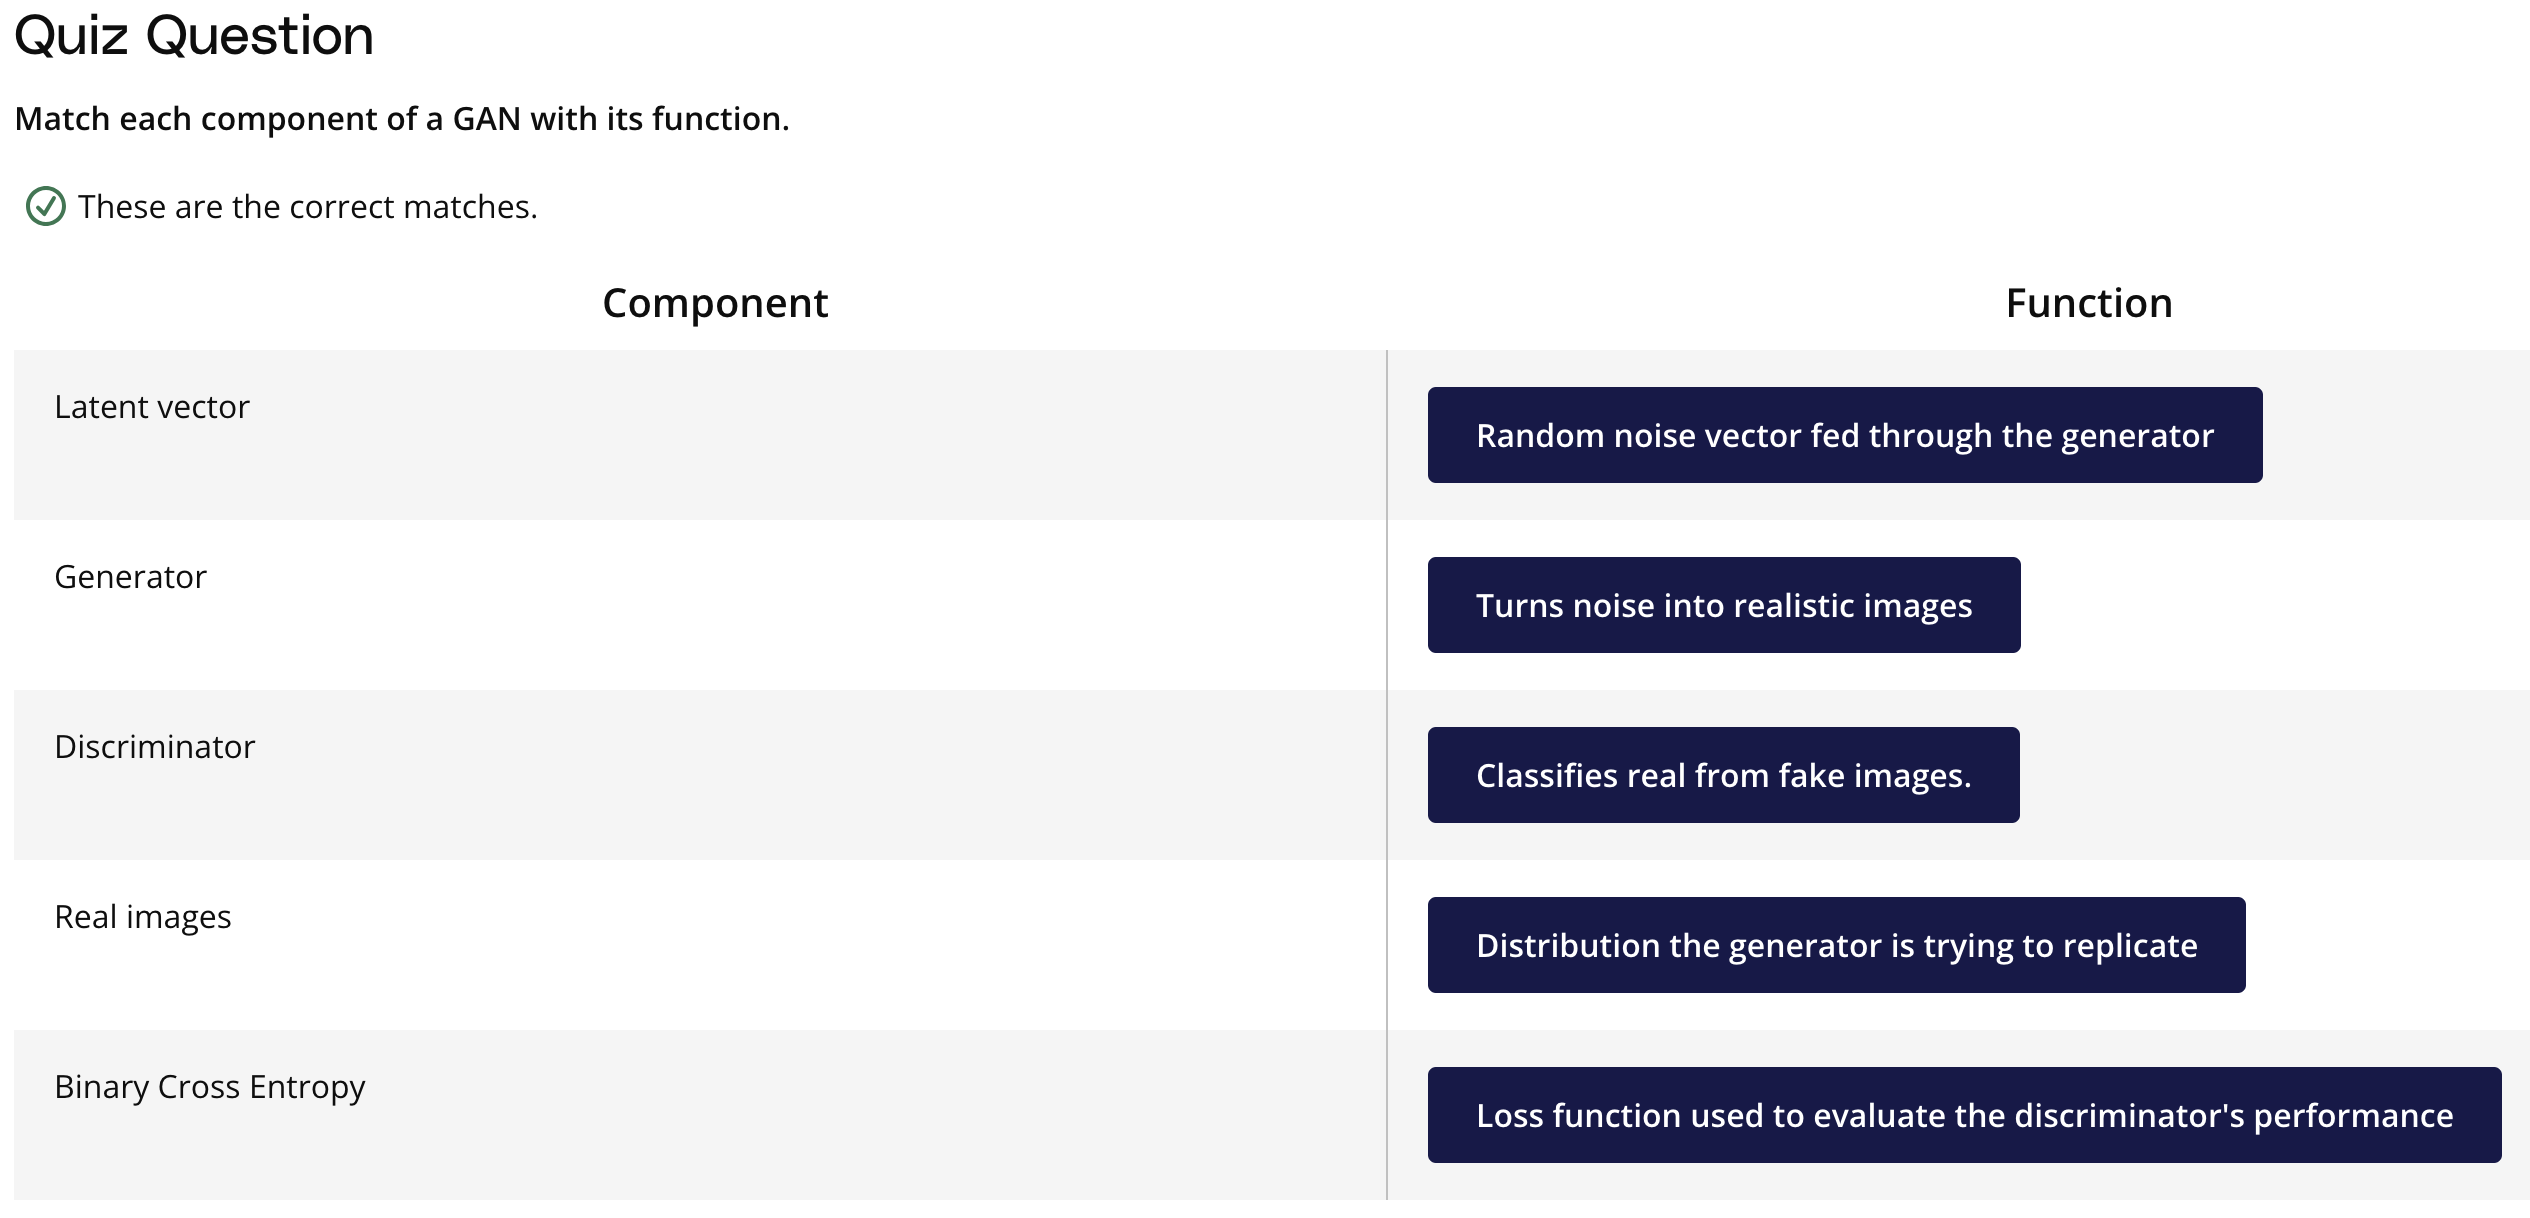
\includegraphics[width=1\linewidth]{img//genAdvNet//gan/quiz3.png}

\section{Generative Adversarial
Network}

In this notebook, we'll be building a generative adversarial network
(GAN) trained on the MNIST dataset. From this, we'll be able to generate
new handwritten digits! We will use the loss functions and models we
built in the previous exercises.

The idea behind GANs is that you have two networks, a generator \(G\)
and a discriminator \(D\), competing against each other. The generator
makes ``fake'' data to pass to the discriminator. The discriminator also
sees real training data and predicts if the data it's received is real
or fake. \textgreater* The generator is trained to fool the
discriminator, it wants to output data that looks \emph{as close as
possible} to real, training data. \textgreater* The discriminator is a
classifier that is trained to figure out which data is real and which is
fake.

What ends up happening is that the generator learns to make data that is
indistinguishable from real data to the discriminator.

The general structure of a GAN is shown in the diagram above, using
MNIST images as data. The latent sample is a random vector that the
generator uses to construct its fake images. This is often called a
\textbf{latent vector} and that vector space is called \textbf{latent
space}. As the generator trains, it figures out how to map latent
vectors to recognizable images that can fool the discriminator.

In this notebook, we will be using the
\href{http://yann.lecun.com/exdb/mnist/}{MNIST Dataset}, a dataset of
handwritten digits. We can use the torch
\href{https://pytorch.org/vision/stable/datasets.html}{Datasets API} to
load the whole dataset directly. The MNIST dataset is made of 28x28
grayscale images.

\begin{lstlisting}[language=Python]
# # run this cell once to install the dependency. 
# You will have to restart the kernel once the package is installed.
!pip install ipywidgets
\end{lstlisting}

\begin{lstlisting}[language=Python]
%matplotlib inline

import numpy as np
import torch
import matplotlib.pyplot as plt
\end{lstlisting}

\begin{lstlisting}[language=Python]
from torchvision import datasets
import torchvision.transforms as transforms

# number of subprocesses to use for data loading
num_workers = 4
# how many samples per batch to load
batch_size = 128

# convert data to torch.FloatTensor
transform = transforms.ToTensor()

# get the training datasets
train_data = datasets.MNIST(root='data', train=True,
                                   download=True, transform=transform)

# prepare data loader
train_loader = torch.utils.data.DataLoader(train_data, 
                                           batch_size=batch_size,
                                           num_workers=num_workers)
\end{lstlisting}

\begin{lstlisting}
/opt/conda/lib/python3.7/site-packages/torchvision/datasets/mnist.py:498: UserWarning: The given NumPy array is not writable, and PyTorch does not support non-writable tensors. This means writing to this tensor will result in undefined behavior. You may want to copy the array to protect its data or make it writable before converting it to a tensor. This type of warning will be suppressed for the rest of this program. (Triggered internally at  ../torch/csrc/utils/tensor_numpy.cpp:178.)
  return torch.from_numpy(parsed.astype(m[2], copy=False)).view(*s)
\end{lstlisting}

\subsubsection{Visualize the data}

We visualize a single random example of the MNIST dataset. You can rerun
this cell multiple times to see different logits.

\begin{lstlisting}[language=Python]
# obtain one batch of training images
rand_index = np.random.randint(0, len(train_data), 1)[0]
images = train_data[rand_index][0]
label = train_data[rand_index][1]
images = images.numpy()

# get one image from the batch
img = np.squeeze(images[0])

fig = plt.figure(figsize = (3,3)) 
ax = fig.add_subplot(111)
ax.imshow(img, cmap='gray')
plt.title(f'Label: {label}')
plt.show()
\end{lstlisting}


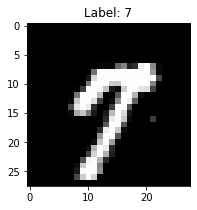
\includegraphics{img/genAdvNet/gan/output_6_0.png}

\section{Define the Model}

A GAN is comprised of two adversarial networks, a discriminator and a
generator. In this exercise, we will be using the Generator and
Discriminator we previously built.

\subsection{Discriminator}

\begin{lstlisting}[language=Python]
import torch.nn as nn
\end{lstlisting}

\begin{lstlisting}[language=Python]
class Discriminator(nn.Module):
    def __init__(self, input_size: int, hidden_dim: int):
        super(Discriminator, self).__init__()
        # define hidden linear layers
        self.fc1 = nn.Linear(input_size, hidden_dim)
        self.fc2 = nn.Linear(hidden_dim, hidden_dim // 2)
        self.fc3 = nn.Linear(hidden_dim // 2, hidden_dim // 4)
        
        # define the final layer
        self.fc4 = nn.Linear(hidden_dim // 4, 1)        
        
        # define the dropout
        self.dropout = nn.Dropout(0.3)
        
        # define the activation
        self.activation = nn.LeakyReLU(0.2)
        
    def forward(self, x: torch.Tensor) -> torch.Tensor:
        # flatten image
        x = x.view(-1, 28*28)
        
        x = self.fc1(x)
        x = self.activation(x)
        x = self.dropout(x)

        x = self.fc2(x)
        x = self.activation(x)
        x = self.dropout(x)

        x = self.fc3(x)
        x = self.activation(x)
        x = self.dropout(x)
        
        # we are using BCE with logits loss so the last activation is not required
        x = self.fc4(x)
        return x
\end{lstlisting}

\subsection{Generator}

\begin{lstlisting}[language=Python]
class Generator(nn.Module):
    def __init__(self, latent_dim: int, hidden_dim: int, output_size: int):
        super(Generator, self).__init__()
        # define hidden linear layers
        self.fc1 = nn.Linear(latent_dim, hidden_dim)
        self.fc2 = nn.Linear(hidden_dim, hidden_dim*2)
        self.fc3 = nn.Linear(hidden_dim*2, hidden_dim*4)
        
        # final fully-connected layer
        self.fc4 = nn.Linear(hidden_dim*4, output_size)
        
        # define the activation
        self.activation = nn.LeakyReLU(0.2)
        self.final_activation = nn.Tanh()

    def forward(self, x: torch.Tensor) -> torch.Tensor:
        x = self.fc1(x)
        x = self.activation(x)

        x = self.fc2(x)
        x = self.activation(x)

        x = self.fc3(x)
        x = self.activation(x)
        
        x = self.fc4(x)
        x = self.final_activation(x)
        return x
\end{lstlisting}

\subsection{Model hyperparameters}

\begin{lstlisting}[language=Python]
# Discriminator hyperparams

# Size of input image to discriminator (28*28)
input_size = 784
# Size of last hidden layer in the discriminator
d_hidden_size = 128

# Generator hyperparams

# Size of latent vector to give to generator
z_size = 100
# Size of discriminator output (generated image)
g_output_size = 784
# Size of first hidden layer in the generator
g_hidden_size = 32
\end{lstlisting}

\subsection{Build complete network}

Now we're instantiating the discriminator and generator from the classes
defined above. Make sure you've passed in the correct input arguments.

\begin{lstlisting}[language=Python]
# instantiate discriminator and generator
D = Discriminator(input_size, d_hidden_size)
G = Generator(z_size, g_hidden_size, g_output_size)

# check that they are as you expect
print(D)
print()
print(G)
\end{lstlisting}

\begin{lstlisting}
Discriminator(
  (fc1): Linear(in_features=784, out_features=128, bias=True)
  (fc2): Linear(in_features=128, out_features=64, bias=True)
  (fc3): Linear(in_features=64, out_features=32, bias=True)
  (fc4): Linear(in_features=32, out_features=1, bias=True)
  (dropout): Dropout(p=0.3, inplace=False)
  (activation): LeakyReLU(negative_slope=0.2)
)

Generator(
  (fc1): Linear(in_features=100, out_features=32, bias=True)
  (fc2): Linear(in_features=32, out_features=64, bias=True)
  (fc3): Linear(in_features=64, out_features=128, bias=True)
  (fc4): Linear(in_features=128, out_features=784, bias=True)
  (activation): LeakyReLU(negative_slope=0.2)
  (final_activation): Tanh()
)
\end{lstlisting}

\subsection{Discriminator and Generator
Losses}

Now we need to calculate the losses. For this exercise, we will use the
loss functions we previously implemented.

\begin{lstlisting}[language=Python]
# Calculate losses
def real_loss(D_out, smooth=False):
    batch_size = D_out.size(0)
    # label smoothing
    if smooth:
        # smooth, real labels = 0.9
        labels = torch.ones(batch_size)*0.9
    else:
        labels = torch.ones(batch_size) # real labels = 1
        
    # numerically stable loss
    criterion = nn.BCEWithLogitsLoss()
    # calculate loss
    loss = criterion(D_out.squeeze(), labels)
    return loss

def fake_loss(D_out):
    batch_size = D_out.size(0)
    labels = torch.zeros(batch_size) # fake labels = 0
    criterion = nn.BCEWithLogitsLoss()
    # calculate loss
    loss = criterion(D_out.squeeze(), labels)
    return loss
\end{lstlisting}

\subsection{Optimizers}

We want to update the generator and discriminator variables separately.
So, we'll define two separate Adam optimizers.

\begin{lstlisting}[language=Python]
import torch.optim as optim

# Optimizers
lr = 0.0002

# Create optimizers for the discriminator and generator
d_optimizer = optim.Adam(D.parameters(), lr)
g_optimizer = optim.Adam(G.parameters(), lr)
\end{lstlisting}

\subsection{Training}

Training will involve alternating between training the discriminator and
the generator. We'll use our functions
\lstinline{real_loss} and
\lstinline{fake_loss} to help us calculate the
discriminator losses in all of the following cases.

\subsubsection{Discriminator training}

\begin{enumerate}
\item Compute the discriminator loss on real, training images
\item Generate fake images
\item Compute the discriminator loss on fake, generated images
\item Add up real and fake loss
\item Perform backpropagation + an optimization step to update the discriminator's weights
\end{enumerate}

\subsubsection{Generator training}

\begin{enumerate}
\item Generate fake images
\item Compute the discriminator loss on fake images, using \textbf{flipped} labels!
\item Perform backpropagation + an optimization step to update the generator's weights
\end{enumerate}

\paragraph{Saving Samples}

As we train, we'll also print out some loss statistics and save some
generated ``fake'' samples.

\begin{lstlisting}[language=Python]
from datetime import datetime
import pickle as pkl
\end{lstlisting}

\begin{lstlisting}[language=Python]
# helper function for viewing a list of passed in sample images
def view_samples(epoch, samples):
    fig, axes = plt.subplots(figsize=(14,4), nrows=2, ncols=8, sharey=True, sharex=True)
    for ax, img in zip(axes.flatten(), samples[epoch]):
        img = img.detach()
        ax.xaxis.set_visible(False)
        ax.yaxis.set_visible(False)
        im = ax.imshow(img.reshape((28,28)), cmap='Greys_r')
    plt.show()
\end{lstlisting}

\begin{lstlisting}[language=Python]
# training hyperparams
num_epochs = 10

# keep track of loss and generated, "fake" samples
samples = []
losses = []

print_every = 100

# Get some fixed data for sampling. These are images that are held
# constant throughout training, and allow us to inspect the model's performance
sample_size = 16
fixed_z = np.random.uniform(-1, 1, size=(sample_size, z_size))
fixed_z = torch.from_numpy(fixed_z).float()

# train the network
D.train()
G.train()
for epoch in range(num_epochs):
    
    for batch_i, (real_images, _) in enumerate(train_loader):
                
        batch_size = real_images.size(0)
        
        ## Important rescaling step ## 
        real_images = real_images*2 - 1  # rescale input images from [0,1) to [-1, 1)
        
        # ============================================
        #            TRAIN THE DISCRIMINATOR
        # ============================================
        d_optimizer.zero_grad()
        
        # 1. Train discriminator on real images & calculate loss
        d_real_outputs = D(real_images)
        d_real_loss = real_loss(d_real_outputs, smooth = True)
        
        # 2. Generate fake images
        # gradients don't have to flow during this step
        with torch.no_grad():
            z = np.random.uniform(-1, 1, size=(batch_size, z_size))
            z = torch.from_numpy(z).float()
            fake_images = G(z)
        
        # 3. Compute the discriminator loss on fake, generated images
        d_fake_outputs = D(fake_images)
        d_fake_loss = fake_loss(d_fake_outputs)
        
        # 4. Add up real and fake loss
        d_loss = d_real_loss + d_fake_loss
        
        # 5. Perform backpropagation + an optimization step to update the discriminator's weights
        d_loss.backward()
        d_optimizer.step()
        
        # =========================================
        #            TRAIN THE GENERATOR
        # =========================================
        g_optimizer.zero_grad()
        
        # 1. Generate fake images
        z = np.random.uniform(-1, 1, size=(batch_size, z_size))
        z = torch.from_numpy(z).float()
        fake_images = G(z)
        
        # 2. Compute the discriminator loss on fake images, using flipped labels!
        g_outputs = D(fake_images)
        g_loss = real_loss(g_outputs)
        
        # 3. Perform backpropagation + an optimization step to update the generator's weights
        g_loss.backward()
        g_optimizer.step()

        # Print some loss stats
        if batch_i % print_every == 0:
            # print discriminator and generator loss
            time = str(datetime.now()).split('.')[0]
            print(f'{time} | Epoch [{epoch+1}/{num_epochs}] | Batch {batch_i}/{len(train_loader)} | d_loss: {d_loss.item():.4f} | g_loss: {g_loss.item():.4f}')
    
            ## AFTER EACH EPOCH##
            # append discriminator loss and generator loss
            losses.append((d_loss.item(), g_loss.item()))
    
    # generate and save sample, fake images
    G.eval() # eval mode for generating samples
    samples_z = G(fixed_z)
    samples.append(samples_z)
    view_samples(-1, samples)
    G.train() # back to train mode


# Save training generator samples
with open('train_samples.pkl', 'wb') as f:
    pkl.dump(samples, f)
\end{lstlisting}

\begin{lstlisting}
2024-08-19 12:38:24 | Epoch [1/10] | Batch 0/469 | d_loss: 1.3956 | g_loss: 0.6160
2024-08-19 12:40:30 | Epoch [1/10] | Batch 100/469 | d_loss: 1.0100 | g_loss: 0.8276
2024-08-19 12:43:06 | Epoch [1/10] | Batch 200/469 | d_loss: 0.9428 | g_loss: 0.9320
2024-08-19 12:45:22 | Epoch [1/10] | Batch 300/469 | d_loss: 0.7070 | g_loss: 1.3122
2024-08-19 12:47:50 | Epoch [1/10] | Batch 400/469 | d_loss: 0.5602 | g_loss: 1.9145
\end{lstlisting}

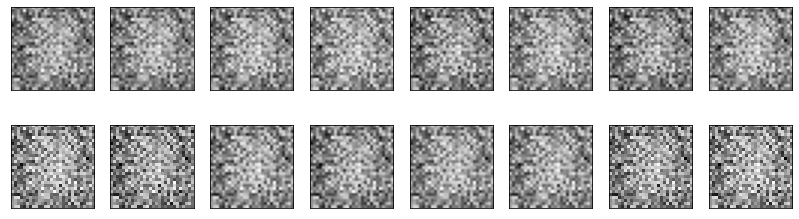
\includegraphics{img/genAdvNet/gan/output_24_1.png}

\begin{lstlisting}
2024-08-19 12:49:35 | Epoch [2/10] | Batch 0/469 | d_loss: 0.4550 | g_loss: 2.6934
2024-08-19 12:51:56 | Epoch [2/10] | Batch 100/469 | d_loss: 0.4889 | g_loss: 2.1672
2024-08-19 12:54:35 | Epoch [2/10] | Batch 200/469 | d_loss: 0.4199 | g_loss: 3.5037
2024-08-19 12:56:44 | Epoch [2/10] | Batch 300/469 | d_loss: 0.3990 | g_loss: 4.0538
2024-08-19 12:59:21 | Epoch [2/10] | Batch 400/469 | d_loss: 0.4340 | g_loss: 3.8504
\end{lstlisting}

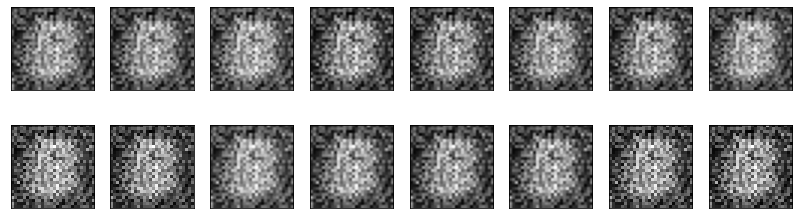
\includegraphics{img/genAdvNet/gan/output_24_3.png}

\begin{lstlisting}
2024-08-19 13:00:19 | Epoch [3/10] | Batch 0/469 | d_loss: 0.4214 | g_loss: 4.2729
2024-08-19 13:01:17 | Epoch [3/10] | Batch 100/469 | d_loss: 0.4621 | g_loss: 5.0454
2024-08-19 13:02:17 | Epoch [3/10] | Batch 200/469 | d_loss: 0.4464 | g_loss: 4.6674
2024-08-19 13:03:14 | Epoch [3/10] | Batch 300/469 | d_loss: 0.5916 | g_loss: 4.5333
2024-08-19 13:04:12 | Epoch [3/10] | Batch 400/469 | d_loss: 0.5599 | g_loss: 4.1011
\end{lstlisting}

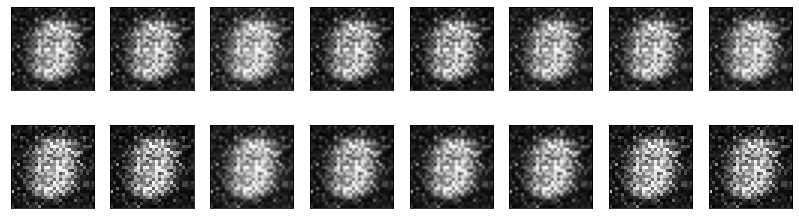
\includegraphics{img/genAdvNet/gan/output_24_5.png}

\begin{lstlisting}
2024-08-19 13:05:01 | Epoch [4/10] | Batch 0/469 | d_loss: 0.4423 | g_loss: 4.7987
2024-08-19 13:06:00 | Epoch [4/10] | Batch 100/469 | d_loss: 0.4567 | g_loss: 5.3195
2024-08-19 13:06:55 | Epoch [4/10] | Batch 200/469 | d_loss: 0.7699 | g_loss: 2.7604
2024-08-19 13:07:54 | Epoch [4/10] | Batch 300/469 | d_loss: 0.6496 | g_loss: 3.0784
2024-08-19 13:08:54 | Epoch [4/10] | Batch 400/469 | d_loss: 0.5625 | g_loss: 3.9456
\end{lstlisting}

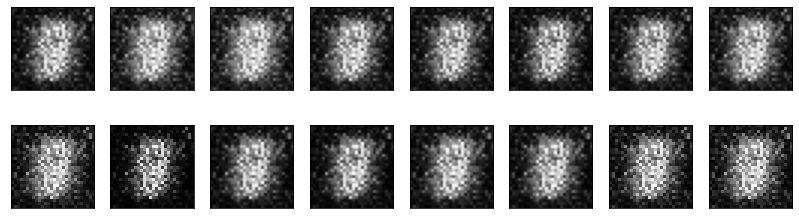
\includegraphics{img/genAdvNet/gan/output_24_7.png}

\begin{lstlisting}
2024-08-19 13:09:35 | Epoch [5/10] | Batch 0/469 | d_loss: 0.4736 | g_loss: 3.5710
2024-08-19 13:10:40 | Epoch [5/10] | Batch 100/469 | d_loss: 0.4453 | g_loss: 4.0432
2024-08-19 13:11:36 | Epoch [5/10] | Batch 200/469 | d_loss: 0.5239 | g_loss: 4.2559
2024-08-19 13:12:36 | Epoch [5/10] | Batch 300/469 | d_loss: 0.5944 | g_loss: 3.4998
2024-08-19 13:13:39 | Epoch [5/10] | Batch 400/469 | d_loss: 0.5396 | g_loss: 4.0217
\end{lstlisting}

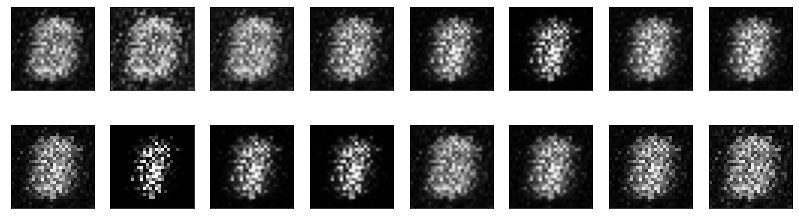
\includegraphics{img/genAdvNet/gan/output_24_9.png}

\begin{lstlisting}
2024-08-19 13:14:29 | Epoch [6/10] | Batch 0/469 | d_loss: 0.5029 | g_loss: 4.0910
2024-08-19 13:15:36 | Epoch [6/10] | Batch 100/469 | d_loss: 0.5573 | g_loss: 5.5966
2024-08-19 13:16:44 | Epoch [6/10] | Batch 200/469 | d_loss: 0.4193 | g_loss: 6.4893
2024-08-19 13:17:52 | Epoch [6/10] | Batch 300/469 | d_loss: 0.4619 | g_loss: 5.3874
2024-08-19 13:19:02 | Epoch [6/10] | Batch 400/469 | d_loss: 0.4260 | g_loss: 5.5646
\end{lstlisting}

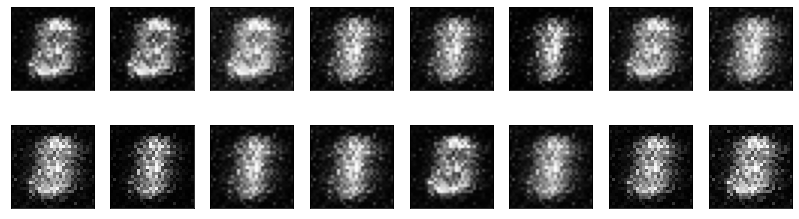
\includegraphics{img/genAdvNet/gan/output_24_11.png}

\begin{lstlisting}
2024-08-19 13:19:51 | Epoch [7/10] | Batch 0/469 | d_loss: 0.4431 | g_loss: 4.8300
2024-08-19 13:21:15 | Epoch [7/10] | Batch 100/469 | d_loss: 0.4341 | g_loss: 4.8061
2024-08-19 13:22:17 | Epoch [7/10] | Batch 200/469 | d_loss: 0.5104 | g_loss: 6.0527
2024-08-19 13:23:16 | Epoch [7/10] | Batch 300/469 | d_loss: 0.5294 | g_loss: 5.6000
2024-08-19 13:24:17 | Epoch [7/10] | Batch 400/469 | d_loss: 0.4048 | g_loss: 5.5299
\end{lstlisting}

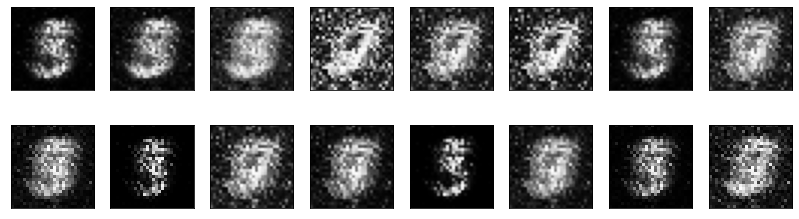
\includegraphics{img/genAdvNet/gan/output_24_13.png}

\begin{lstlisting}
2024-08-19 13:25:05 | Epoch [8/10] | Batch 0/469 | d_loss: 0.4675 | g_loss: 4.7217
2024-08-19 13:26:11 | Epoch [8/10] | Batch 100/469 | d_loss: 0.4515 | g_loss: 4.9083
2024-08-19 13:27:28 | Epoch [8/10] | Batch 200/469 | d_loss: 0.4682 | g_loss: 5.4478
2024-08-19 13:28:49 | Epoch [8/10] | Batch 300/469 | d_loss: 0.4417 | g_loss: 6.2993
2024-08-19 13:30:06 | Epoch [8/10] | Batch 400/469 | d_loss: 0.4591 | g_loss: 3.9562
\end{lstlisting}

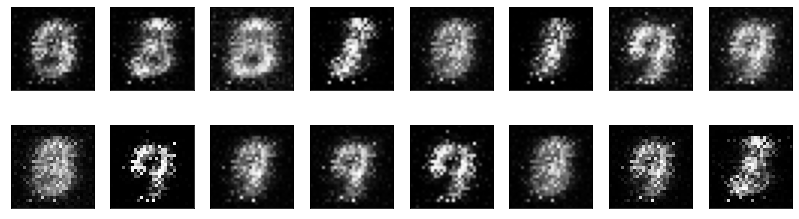
\includegraphics{img/genAdvNet/gan/output_24_15.png}

\begin{lstlisting}
2024-08-19 13:31:01 | Epoch [9/10] | Batch 0/469 | d_loss: 0.5769 | g_loss: 4.4656
2024-08-19 13:32:14 | Epoch [9/10] | Batch 100/469 | d_loss: 0.5056 | g_loss: 4.3632
2024-08-19 13:33:27 | Epoch [9/10] | Batch 200/469 | d_loss: 0.4482 | g_loss: 4.9012
2024-08-19 13:34:40 | Epoch [9/10] | Batch 300/469 | d_loss: 0.5288 | g_loss: 5.1727
2024-08-19 13:35:59 | Epoch [9/10] | Batch 400/469 | d_loss: 0.5007 | g_loss: 4.8494
\end{lstlisting}

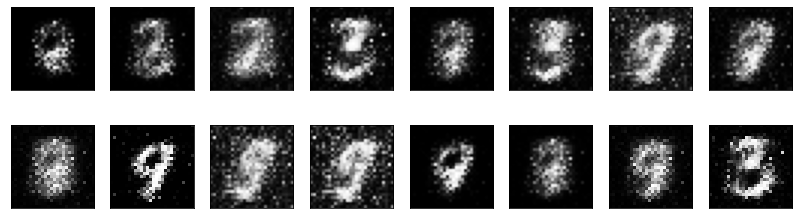
\includegraphics{img/genAdvNet/gan/output_24_17.png}

\begin{lstlisting}
2024-08-19 13:36:59 | Epoch [10/10] | Batch 0/469 | d_loss: 0.5755 | g_loss: 4.2650
2024-08-19 13:38:15 | Epoch [10/10] | Batch 100/469 | d_loss: 0.6573 | g_loss: 3.2818
2024-08-19 13:39:26 | Epoch [10/10] | Batch 200/469 | d_loss: 0.5454 | g_loss: 4.2313
2024-08-19 13:40:26 | Epoch [10/10] | Batch 300/469 | d_loss: 0.6774 | g_loss: 4.5947
2024-08-19 13:41:27 | Epoch [10/10] | Batch 400/469 | d_loss: 0.6092 | g_loss: 3.5220
\end{lstlisting}

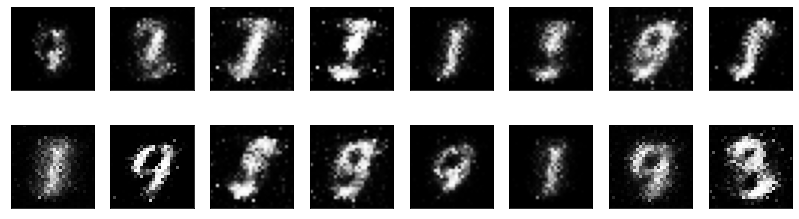
\includegraphics{img/genAdvNet/gan/output_24_19.png}

\subsection{Training loss}

Here we'll plot the training losses for the generator and discriminator,
recorded after each epoch.

\begin{lstlisting}[language=Python]
fig, ax = plt.subplots()
losses = np.array(losses)
plt.plot(losses.T[0], label='Discriminator')
plt.plot(losses.T[1], label='Generator')
plt.title("Training Losses")
plt.legend()
\end{lstlisting}

\begin{lstlisting}
<matplotlib.legend.Legend at 0x799d977663d0>
\end{lstlisting}

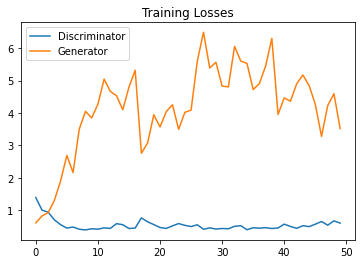
\includegraphics{img/genAdvNet/gan/output_26_1.png}

\subsection{Generator samples from
training}

Here we can view samples of images from the generator. First we'll look
at the images we saved during training.

\begin{lstlisting}[language=Python]
# Load samples from generator, taken while training
with open('train_samples.pkl', 'rb') as f:
    samples = pkl.load(f)
\end{lstlisting}

These are samples from the final training epoch. You can see the
generator is able to reproduce numbers like 1, 7, 3, 2. Since this is
just a sample, it isn't representative of the full range of images this
generator can make.

\begin{lstlisting}[language=Python]
# -1 indicates final epoch's samples (the last in the list)
view_samples(-1, samples)
\end{lstlisting}

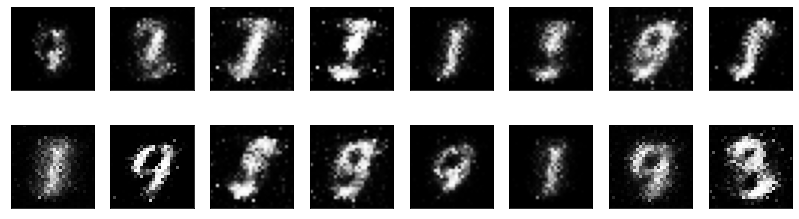
\includegraphics{img/genAdvNet/gan/output_30_0.png}

Below I'm showing the generated images as the network was training,
every 10 epochs.

\begin{lstlisting}[language=Python]
rows = 10 # split epochs into 10, so 100/10 = every 10 epochs
cols = 6
fig, axes = plt.subplots(figsize=(7,12), nrows=rows, ncols=cols, sharex=True, sharey=True)

for sample, ax_row in zip(samples[::int(len(samples)/rows)], axes):
    for img, ax in zip(sample[::int(len(sample)/cols)], ax_row):
        img = img.detach()
        ax.imshow(img.reshape((28,28)), cmap='Greys_r')
        ax.xaxis.set_visible(False)
        ax.yaxis.set_visible(False)
\end{lstlisting}

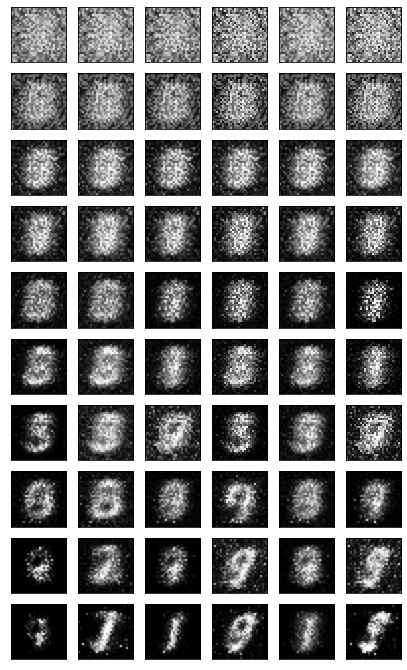
\includegraphics{img/genAdvNet/gan/output_32_0.png}

It starts out as all noise. Then it learns to make only the center white
and the rest black. You can start to see some number like structures
appear out of the noise like 1s and 9s.

\subsection{Sampling from the generator}

We can also get completely new images from the generator by using the
checkpoint we saved after training. \textbf{We just need to pass in a
new latent vector \(z\) and we'll get new samples}!

\begin{lstlisting}[language=Python]
# randomly generated, new latent vectors
sample_size = 16
rand_z = np.random.uniform(-1, 1, size=(sample_size, z_size))
rand_z = torch.from_numpy(rand_z).float()

G.eval() # eval mode
# generated samples
rand_images = G(rand_z)

# 0 indicates the first set of samples in the passed in list
# and we only have one batch of samples, here
view_samples(0, [rand_images])
\end{lstlisting}

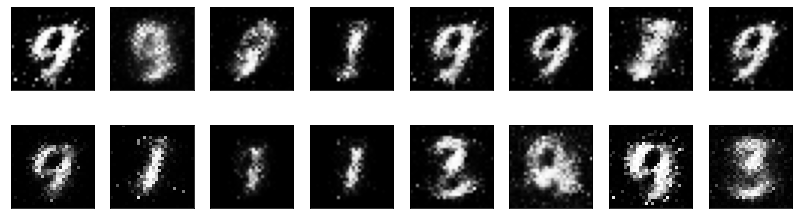
\includegraphics{img/genAdvNet/gan/output_35_0.png}

\section{Exercise Part 3: Solution}
\href{https://www.youtube.com/watch?v=HdhMtWz68Vo}{Youtube}
